\documentclass[a4paper]{article} 
\addtolength{\hoffset}{-2.25cm}
\addtolength{\textwidth}{4.5cm}
\addtolength{\voffset}{-3.25cm}
\addtolength{\textheight}{5cm}
\setlength{\parskip}{0pt}
\setlength{\parindent}{0in}

\usepackage{blindtext} % Package to generate dummy text
\usepackage{charter} % Use the Charter font
\usepackage[utf8]{inputenc} % Use UTF-8 encoding
\usepackage{microtype} % Slightly tweak font spacing for aesthetics
\usepackage[english]{babel} % Language hyphenation and typographical rules
\usepackage{amsthm, amsmath, amssymb} % Mathematical typesetting
\usepackage{float} % Improved interface for floating objects
\usepackage[final, colorlinks = true, 
linkcolor = black, 
citecolor = black]{hyperref} % For hyperlinks in the PDF
\usepackage{graphicx, multicol} % Enhanced support for graphics
\usepackage{xcolor} % Driver-independent color extensions
\usepackage{marvosym, wasysym} % More symbols
\usepackage{rotating} % Rotation tools
\usepackage{subcaption}
\usepackage{censor} % Facilities for controlling restricted text
\newcommand{\note}[1]{\marginpar{\scriptsize \textcolor{red}{#1}}} % Enables comments in red on margin
\usepackage{bm}
\usepackage{blkarray}
\usepackage{enumitem}
\usepackage{pgfplots}
\definecolor{colkeyword}{rgb}{0,0.4,0}
\definecolor{colname}{rgb}{0.4,0.4,0}
\definecolor{coltype}{rgb}{0.4,0,0.4}
\definecolor{coloperators}{rgb}{0,0,1.0}
\definecolor{colscopes}{rgb}{0.4,0,0}

\setcounter{tocdepth}{2}
% Title Page
\title{Summary Machine Learning 1}
\author{Phillip Lippe}


\begin{document}
\maketitle
\tableofcontents
\newpage

\section{Probability Theory}
\subsection{Multivariate Gaussian}
$$\mathcal{N}\left(\bm{x}|\bm{\mu}, \bm{\Sigma}\right) = \frac{1}{\left(2\pi\right)^{D/2} \cdot |\bm{\Sigma}|^{1/2}}\cdot \exp\left(-\frac{1}{2}\left(\bm{x}-\bm{\mu}\right)^T\bm{\Sigma}^{-1}\left(\bm{x}-\bm{\mu}\right)\right)$$

$$\frac{\partial}{\partial \bm{\mu}}\mathcal{N}\left(\bm{x}|\bm{\mu}, \bm{\Sigma}\right)  = \mathcal{N}\left(\bm{x}|\bm{\mu}, \bm{\Sigma}\right) \left(\bm{x}-\bm{\mu}_k\right)^T\bm{\Sigma}^{-1}$$

% $$\frac{\partial}{\partial \bm{\Sigma}}\mathcal{N}\left(\bm{x}|\bm{\mu}, \bm{\Sigma}\right)  = ...$$

\subsection{Rules of probability}
\begin{table}[ht]
	\centering
	\begin{tabular}{c|cc}
		& \textbf{Discrete} & \textbf{Continuous}\\
		\hline
		\textbf{Additivity} & $p(X\in A) = \sum\limits_{x\in A}p(x)$ & $p\left(x\in (a,b)\right) = \int\limits_{a}^{b}p(x)dx$\\[10pt]
		\textbf{Positivity} & $0 \leq p(x)\leq 1$ & $0 \leq p(x) \not\leq 1$\\[10pt]
		\textbf{Normalization} & $\sum_{x} p(x) = 1$ & $\int_{\chi} p(x)dx = 1$\\[10pt]
		\textbf{Sum Rule} & $p(x) = \sum\limits_{y\in\mathcal{Y}} p(x,y)$ & $p(x)=\int\limits p(x,y)dy$\\[10pt]
		\textbf{Product Rule} & $p(x,y) = p(x|y)p(y)$ & $p(x,y) = p(x|y)p(y)$
	\end{tabular}
\end{table}
\subsection{Bayes Rule}
$$\underbrace{p(x|y)}_{\text{posterior}} = \frac{\overbrace{p(y|x)}^{\text{likelihood}} \overbrace{p(x)}^{\text{prior}}}{\underbrace{p(y)}_{\text{evidence}}} = \frac{p(y|x) p(x)}{\int p(y|x) p(x)dx} \text{\hspace{5mm}or\hspace{5mm}} \frac{p(y|x) p(x)}{\sum p(y|x) p(x)}$$
\section{Linear Regression}

\subsection{Basic approaches}
\subsubsection{Maximum likelihood}
\begin{itemize}
	\item Given a dataset $D=(\bm{x}_1, \bm{x}_2, ..., \bm{x}_N)$ of $N$ independent observations
	\item The likelihood of the dataset given the model parameters $\bm{w}$ is specified as $p(D|\bm{w})$
	\item \textit{Maximum likelihood estimation}: the most likely ``explanation'' of $D$ is $\bm{w}_{\text{ML}}$:
	$$\bm{w}_{\text{ML}} = \arg\max_{\bm{w}} p(D|\bm{w})$$
	\item Using the i.i.d. assumption, we can state $p(D|\bm{w}) = \prod\limits_{n=1}^{N} p(\bm{x}_n|\bm{w})$
	\item For preventing numerical overflow and mostly simplifying the derivation, we can take the logarithm $\log p(D|\bm{w})$
	\item Maximum where $\frac{\partial}{\partial \bm{w}}\log p(D|\bm{w}) = 0$
	\item We can check whether our estimation is biased by comparing the expected result by the distribution parameters: $$\mathbb{E}\left[\sigma_{ML}^{2}\right] = \mathbb{E}\left[\frac{1}{N}\sum\limits_{i=1}^{N}\left(x_i - \frac{1}{N}\sum_{n=1}^{N} x_n\right)^2\right] = \frac{N-1}{N} \sigma^2 \implies \text{biased estimator}$$
\end{itemize}
\subsubsection{Maximum a posteriori}
\begin{itemize}
	\item Choose the most probable model parameters $\bm{w}$ given data $D$:
	$$\bm{w}_{\text{MAP}} = \arg\max_{\bm{w}} p(\bm{w}|D)$$
	\item By applying the Bayes rule (and log), we get:
	$$\bm{w}_{\text{MAP}} = \arg\max_{\bm{w}} \log p(D|\bm{w}) + \log p(\bm{w}) - \log p(D)$$
	\item We can drop the evidence as it is independent of $\bm{w}$
\end{itemize}
\subsubsection{Bayesian approach}
\begin{itemize}
	\item Frequentist approaches only consider point estimates without taking the uncertainty of the prediction into account
	\item Given a prior belief over $\bm{w}$, we are interested in the posterior distribution (not only maximum!)
	\item The predictive distribution for a new data point $\bm{x}'$ is therefore 
	$$p(t'|\bm{x}',D) = \int p(t'| \bm{x}', \bm{w}) \cdot p(\bm{w}|D) d\bm{w}$$
	\item Thus, we also consider our uncertainty when predicting
	\item However, we need to compute the evidence for that which is mostly quite hard (prefer less complex models)
\end{itemize}
\subsection{Model selection for supervised learning}
\begin{itemize}
	\item Model selection comes with two main questions:
	\begin{enumerate}
		\item How can we estimate the performance of a model on unknown data?
		\item How can we choose the optimal hyperparameters? $\Rightarrow$ \textbf{model selection}
	\end{enumerate}
	\item Common approach for large datasets: split in train, val and test dataset
	\begin{description}
		\item[Training dataset] About 80\% of the data should be used for training. On this, we try to minimize the error/loss $L\left(y(\bm{x}_i),t_i\right)$ for $(\bm{x},t)\in D_{train}$ and find optimal parameters $\bm{w}^*$.
		\item[Validation dataset] About 10\% of the data is used for estimating the test error $L\left(y(\bm{x}_{\text{val}}, \bm{w}^*),t_{\text{val}}\right)$ for various $\bm{w}^*$ from different hyperparameters. Hence, the hyperparameters are tuned on the validation dataset.
		\item[Testing dataset] The last 10\% of the available data provides the final test of the chosen best weights and hyperparameters. This data is used to estimate the performance on unseen data, and should therefore not be used for any parameter choosing!
	\end{description}
	\item However, for a small dataset, the validation and test set is very small and, hence, very noisy $\Rightarrow$ use cross validation
\end{itemize}
\subsubsection{Cross Validation}
\begin{itemize}
	\item Split data into $K$ folds % $D=\left\{\left(x_1, t_1\right), \left(x_2, t_2\right), ..., \left(x_N, t_N\right)\right\}$
	\item If $K=N$, it is also called leave-one-out cross validation as the validation is one single data point
	\item Train the model $y$ on $K-1$ folds, and test on the remaining fold $k$ $\Rightarrow$ model $\hat{y}^{\mbox{--}k}(x)$
	\item The estimation of the prediction error is the mean validation error over all folds. With the index function $\kappa:\left\{1,...,N\right\}\mapsto\left\{1,...,K\right\}$ (mapping data point to corresponding fold where it is used for validation), we get:
	$$CV(\hat{y}) = \frac{1}{N}\sum\limits_{i=1}^{N}L\left(\hat{y}^{\mbox{--}\kappa\left(i\right)}(\bm{x}_i), t_i\right)$$
	\item Task of model selection: Run cross validation for each possible parameter setting and choose the one with lowest cross validation error
	\item Task of test error estimation: after finding the best hyperparameters like $\alpha^*$, retrain model on all $K$ folds, and test this model on a held-out test set
	\item However, if test set is small, we again get a noisy estimation $\Rightarrow$ Nested cross validation
	\item Drawback of cross validation: it is computationally expensive and should therefore only be used for fast trainings/small datasets
\end{itemize}
\subsubsection{Nested Cross Validation}
\begin{itemize}
	\item Cross validation for both model selection and model performance by reusing dataset for testing
	\item General algorithm:
	\begin{enumerate}
		\item Split dataset into $M$ cross validation folds
		\item For each of these folds $m=1,...,M$:
		\begin{enumerate}
			\item Let fold $m$ be the test dataset
			\item Apply cross validation on the remaining data by splitting it into $K$ folds and find best hyperparameters $\alpha^*,\beta^*,...$
			\item Retrain the model with the best hyperparameters on all data besides the fold $m$
			\item Test the model on unseen data fold $m$ 
		\end{enumerate}
		\item The final generalization error/loss on unseen data is the mean over all $M$ folds
	\end{enumerate}
	\item For choosing the best hyperparameters $\alpha^*,\beta^*,...$, we use single cross validation on the whole dataset again without a test dataset, but record the found generalization error as estimation for unknown data, also for the new model
\end{itemize}
\begin{figure}[ht]
	\centering
	\includegraphics[width=0.5\textwidth]{figures/cross_validation_nested.png}
	\caption{Illustration of nested cross validation. The outer loop splits dataset into test and trainval parts. Within the trainval parts, we apply cross validation to find optimal hyperparameters. Those are tested on the left-out fold from the outer loop, and the mean test error of all folds is the final generalization error. Note that every outer fold can lead to different optimal hyperparameters.}
	\label{img:linear_regression_nested_cross_validation}
\end{figure}
\subsection{Bias variance decomposition}
\begin{itemize}
	\item Frequentist view on model complexity
	\item Common loss: the squared loss function, defined as $L\left(t, y\left(\bm{x}\right)\right) = \left(t - y\left(\bm{x}\right)\right)^2$
	% \item The expected loss is $\mathbb{E}\left[L\left(t, y\left(\bm{x}\right)\right)\right]=\int\int \left(t - y\left(\bm{x}\right)\right)^2 p\left(\bm{x}, t\right) \text{d}\bm{x} \text{ d}t$
	\item An optimal model of $y\left(\bm{x}\right)$ would minimize this loss which is given by $$h(\bm{x}) = \mathbb{E}\left[t|\bm{x}\right] = \int t\cdot p\left(t|\bm{x}\right) \text{d}t$$
	where the conditional distribution $p\left(t|\bm{x}\right)$ is the actual, noisy data distribution (not known!)
	\item Thus, the expected squared loss can be written as
	$$\mathbb{E}\left[L\right] = \int\underbrace{\left\{y(\bm{x}) - \mathbb{E}\left[t|\bm{x}\right]\right\}^2}_{\text{model loss}} p(\bm{x}) \text{d}\bm{x} + \int\underbrace{\left\{\mathbb{E}\left[t|\bm{x}\right] - t\right\}^2}_{\text{intrinsic noise on data}} p(\bm{x},t) \text{d}\bm{x}\text{ d}t$$
	where the first term, the model loss, depends on how different the model $y(\bm{x})$ is from the actual data distribution, and the second term arises from the intrinsic noise and represents the minimum achievable expected loss
	\item In Bayesian approach, we would model $y(\bm{x}, \bm{w})$ where the uncertainty of $\bm{w}$ is expressed in the posterior distribution
	\item However, from a frequentist viewpoint, we use multiple datasets $\mathcal{D}$ on which we train our model and get a single estimation $\bm{\hat{w}}$ for each of them. The final model is the average over this ensemble of datasets.
	\item To apply this approach, we take the model loss for a single input $\bm{x}$, and add the expected model over all datasets:
	\begin{equation*}
		\begin{split}
			\left\{y\left(\bm{x};\mathcal{D}\right) - h\left(\bm{x}\right)\right\}^2 & = \left\{y\left(\bm{x};\mathcal{D}\right) - \mathbb{E}_{\mathcal{D}}\left[y\left(\bm{x};\mathcal{D}\right)\right] + \mathbb{E}_{\mathcal{D}}\left[y\left(\bm{x};\mathcal{D}\right)\right] - h\left(\bm{x}\right)\right\}^2\\
			& = \left\{y\left(\bm{x};\mathcal{D}\right) - \mathbb{E}_{\mathcal{D}}\left[y\left(\bm{x};\mathcal{D}\right)\right]\right\}^2 + \left\{\mathbb{E}_{\mathcal{D}}\left[y\left(\bm{x};\mathcal{D}\right)\right] - h\left(\bm{x}\right)\right\}^2 \\
			& \text{\hspace{5mm} } + 2\left\{y\left(\bm{x};\mathcal{D}\right) - \mathbb{E}_{\mathcal{D}}\left[y\left(\bm{x};\mathcal{D}\right)\right]\right\}\left\{ \mathbb{E}_{\mathcal{D}}\left[y\left(\bm{x};\mathcal{D}\right)\right] - h\left(\bm{x}\right)\right\}
		\end{split}
	\end{equation*}
	\item The final model of the frequentist approach is the expected value of this loss over all datasets:
	\begin{equation*}
		\begin{split}
			\mathbb{E}_{\mathcal{D}}\left[\left\{y\left(\bm{x};\mathcal{D}\right) - h\left(\bm{x}\right)\right\}^2\right] & = \underbrace{\mathbb{E}_{\mathcal{D}}\left[\left\{y\left(\bm{x};\mathcal{D}\right) - \mathbb{E}_{\mathcal{D}}\left[y\left(\bm{x};\mathcal{D}\right)\right]\right\}^2\right]}_{\text{\textcolor{red}{variance}}} + \underbrace{\left\{\mathbb{E}_{\mathcal{D}}\left[y\left(\bm{x};\mathcal{D}\right)\right] - h(\bm{x})\right\}^2}_{\textcolor{blue}{(\text{bias})^2}}
		\end{split}
	\end{equation*}
	where the first term is the \textbf{variance} of a model trained on a single dataset compared to the average, and the second term is the loss of the average/expected model over all datasets, or rather the \textbf{bias} of the model. The third term of the original equation is eliminated as only $y(\bm{x};\mathcal{D})$ is affected by the expectation operator $\mathbb{E}_{\mathcal{D}}$, and is the same as $\mathbb{E}_{\mathcal{D}}\left[y\left(\bm{x};\mathcal{D}\right)\right]$. 
	\item Coming back to the original expected squared loss, we can decompose it into three terms:
	$$\text{expected loss} = (\text{bias})^2 + \text{variance} + \text{noise}$$
	where
	\begin{equation*}
		\begin{split}
			(\text{bias})^2 &= \int \left\{\mathbb{E}_{\mathcal{D}}\left[y\left(\bm{x};\mathcal{D}\right)\right] - h(\bm{x})\right\}^2p(\bm{x}) \text{d}\bm{x}\\
			\text{variance} &= \int \mathbb{E}_{\mathcal{D}}\left[\left\{y\left(\bm{x};\mathcal{D}\right) - \mathbb{E}_{\mathcal{D}}\left[y\left(\bm{x};\mathcal{D}\right)\right]\right\}^2\right]p(\bm{x}) \text{d}\bm{x}\\
			\text{noise} &= \int \left\{h(\bm{x})-t\right\}^2p\left(\bm{x},t\right)\text{d}\bm{x}\text{ d}t
		\end{split}
	\end{equation*}
	\item Now, the task is to find the best balance between bias and variance. An example for the data distribution $\mathbb{E}[t|x]=\sin(2\pi x)$ (note that noise is canceled by expectation), 24 Gaussian basis functions and regularized loss function is shown in Figure~\ref{img:linear_regression_bias_variance_decomp_example}.
	\begin{figure}[ht]
		\centering
		\includegraphics[width=0.4\textwidth]{figures/bias_variance_reg_comp.png}
		\caption{Illustration of dependence of bias and variance on model complexity controlled by $\lambda$. Less complex models (high $\lambda$) tend to have a high bias (be far off the correct distribution) but it is more robust regarding the actual dataset (therefore, a low variance). Decreasing $\lambda$ results in a lower bias, but a high variance as models tend to overfit and are therefore sensitive to the dataset.}
		\label{img:linear_regression_bias_variance_decomp_example}
	\end{figure}
	\item Plotting the terms of the decomposed squared loss function over $\lambda$ gives further insights of the model behavior (see Figure~\ref{img:linear_regression_bias_variance_decomp_error_plot}). For generating such a plot, the integrals are approximated by sums over all data points $x$ as we have a limited number of samples.
	\begin{figure}[ht]
		\centering
		\includegraphics[width=0.4\textwidth]{figures/bias_variance_loss_plot.png}
		\caption{Plot of decomposed loss function for example of Figure~\ref{img:linear_regression_bias_variance_decomp_example}. The goal is to minimize the test error. It is common that this is close to the minimum value of $(\text{bias})^2+\text{variance}$. High variance as on the left indicates overfitting, high bias error on the left shows that the model is underfitting.}
		\label{img:linear_regression_bias_variance_decomp_error_plot}
	\end{figure}
	\item In conclusion, high values of $\lambda$ reduce model complexity, and therefore increase bias loss and leads to underfitting. However, it provides a small variance.\\In contrast, small values of $\lambda$ causes a low bias as the model is quite complex. Still, the variance is high indicating that the model overfits on the small datasets.
	\item The bias-variance decomposition is less practical as it is better to train on one large dataset instead of splitting it into several small ones. Furthermore, this reduces the risk of overfitting for a high model complexity on the data anyways.
\end{itemize}
\subsection{Bayesian Linear Regression}
\begin{itemize}
	\item Determining the suitable model complexity using the training data alone without overfitting
	\item Result is a distribution of $\bm{w}$ instead of single value as in maximum likelihood or posterior
\end{itemize}
\subsubsection{Parameter distribution}
\begin{itemize}
	\item Prior over weights: $p(\bm{w}) = \mathcal{N}\left(\bm{m}_0, \bm{S}_0\right)$
	\item Likelihood: $p\left(t'|\bm{x}', \bm{w}, \beta\right)=\mathcal{N}\left(t'|\bm{\phi}(\bm{x})^T\bm{w}, \beta^{-1}\right)$
	\item Posterior distribution: $p(\bm{w}|\bm{t}, \bm{X}) = \frac{p\left(\bm{t}|\bm{X}, \bm{w}, \beta\right) p\left(\bm{w}\right)}{p\left(\bm{t}|\bm{X}, \beta\right)} = \mathcal{N}\left(\bm{m}_N, \bm{S}_N\right)$, where\\
	$$\bm{S}_N^{-1}=\bm{S}_0^{-1} + \beta \bm{\Phi}^T\bm{\Phi}$$
	$$\bm{m}_N = \bm{S}_N\left(\bm{S}_0^{-1}\bm{m}_0+\beta\bm{\Phi}^T\bm{t}\right)$$
	\item Maximum a posteriori corresponds by $\bm{w}_{\text{MAP}} = \bm{m}_N$
	\item If no prior was given ($\bm{S}_0=\alpha^{-1} \bm{I}$ with $\alpha\to0$) the mean $\bm{m}_N$ reduces to $\bm{w}_{\text{ML}}$
	\item Mostly simpler Gaussian prior used: $p(\bm{w}) = \mathcal{N}\left(\bm{0}, \alpha^{-1}\bm{I}\right)$
	\begin{itemize}
		\item Resulting parameters of posterior: 
		$$\bm{S}_N^{-1}=\alpha^{-1}\bm{I} + \beta \bm{\Phi}^T\bm{\Phi}$$
		$$\bm{m}_N = \beta \bm{S}_N\bm{\Phi}^T\bm{t}$$
		$$p(\bm{w}|\bm{t}, \bm{X})=\frac{1}{\sqrt{\left(2\pi\right)^M |\bm{S}_N|}}\exp\left[-\frac{1}{2}\left(\bm{w}-\bm{m}_N\right)^T \bm{S}_N^{-1} \left(\bm{w}-\bm{m}_N\right)\right]$$
		\item Corresponding log posterior: 
		$$\ln p\left(\bm{w}|\bm{t}, \bm{X}\right) = -\frac{\beta}{2}\sum\limits_{n=1}^{N}\left\{t_n - \bm{w}^T \bm{\phi}\left(\bm{x}_n\right)\right\}^2 - \frac{\alpha}{2}\bm{w}^T \bm{w} + C$$
		\item Thus, maximizing this posterior is equal to having a regularization term with $\lambda=\frac{\alpha}{\beta}$
		\item Infinitely narrow prior by $\alpha\to\infty$ ($\alpha\to0$ seen before ends up in maximum likelihood):
		$$\lim\limits_{\alpha\to\infty} \bm{S}_N = \lim\limits_{\alpha\to\infty} \left(\alpha\bm{I}+\beta \bm{\Phi}^{T}\bm{\Phi}\right)^{-1} = \lim\limits_{\alpha\to\infty} \alpha^{-1}\bm{I} = \bm{0}$$
		$$\lim\limits_{\alpha\to\infty} \bm{m}_N = \lim\limits_{\alpha\to\infty} \beta\left(\alpha\bm{I}+\beta \bm{\Phi}^{T}\bm{\Phi}\right)^{-1}\bm{\Phi}^T \bm{t} = \lim\limits_{\alpha\to\infty} \frac{\beta}{\alpha}\bm{\Phi}^T\bm{t} = \bm{0} = \bm{m}_{0}$$
		\item Infinite data $N\to\infty$:
		$$\lim\limits_{N\to\infty} \bm{S}_N = \lim\limits_{N\to\infty} \left(\alpha\bm{I}+\beta \bm{\Phi}^{T}\bm{\Phi}\right)^{-1} = \lim\limits_{N\to\infty} \left(\bm{\Phi}^{T}\bm{\Phi}\right)^{-1} = \bm{0}$$
		$$\lim\limits_{N\to\infty} \bm{m}_N = \lim\limits_{N\to\infty} \beta\left(\alpha\bm{I}+\beta \bm{\Phi}^{T}\bm{\Phi}\right)^{-1}\bm{\Phi}^T \bm{t} = \lim\limits_{N\to\infty} \left(\bm{\Phi}^T\bm{\Phi}\right)^{-1}\bm{\Phi}^T\bm{t} = \bm{w}_{\text{ML}}$$
		$\Rightarrow$ At infinite data, all approaches agree: $\bm{m}_N = \bm{w}_{\text{ML}} = \bm{w}_{\text{MAP}}$
	\end{itemize}
\end{itemize}

\subsubsection{Sequential Bayesian Learning}
\begin{itemize}
	\item Data is sequences of input $x$ and target $t$
	\item Posterior after $N-1$ data points constitutes the prior for the $N$th data point!
	\item Posterior 1: $p(\bm{w}|x_1,t_1,\alpha,\beta)\propto p(t_1|x_1,\bm{w},\beta)p(\bm{w}|\alpha)$
	\item Posterior 2: $p\left(\bm{w}|(x_1,t_1),(x_2,t_2),\alpha,\beta\right)\propto p(t_2|x_2,\bm{w},\beta)p(\bm{w}|x_1,t_1,\alpha,\beta)$
	\item Posterior narrows down step by step until it gets very certain of the correct estimation 
\end{itemize}
\begin{figure}[ht]
\centering
\includegraphics[width=0.5\textwidth]{figures/sequential_bayesian_linear_regression.png}
\caption{Example for Sequential Bayesian Learning on target $t=-0.3+0.5x+\epsilon$. First column: likelihood (not normalized for $\bm{w}$, but for $t_n$!), second column: posterior, third column: sampled weights}
\end{figure}
\subsubsection{Predictive Distribution}
\begin{itemize}
	\item Predictive distribution is defined by ($\bm{\mathtt{t}}$ targets in training set):
	$$p\left(t|x, \bm{\mathtt{t}}, \bm{X}, \alpha, \beta \right) = \int p\left(t|x, \bm{w},\beta\right)p\left(\bm{w}|\bm{\mathtt{t}}, \bm{X}, \alpha, \beta\right)d\bm{w}$$
	where $p\left(t|x, \bm{w},\beta\right) = \mathcal{N}\left(t|y\left(\bm{x},\bm{w}\right), \beta^{-1}\right)$ is the conditional distribution of target variable, and \\$p\left(\bm{w}|\bm{\mathtt{t}}, \bm{X}, \alpha, \beta\right) = \mathcal{N}\left(\bm{w}|\bm{m}_N, \bm{S}_N\right)$ the posterior weight distribution
	\item Predictive distribution is convolution of two Gaussians $\Rightarrow$ $p\left(t|x, \bm{\mathtt{t}}, \bm{X}, \alpha, \beta \right)=\mathcal{N}\left(t|\bm{m}_N^{T}\bm{\phi}(\bm{x}),\sigma_N^2(\bm{x}) \right)$
	where variance $\sigma_N^2(\bm{x})=\frac{1}{\beta} + \bm{\phi}(\bm{x})^T \bm{S}_N \bm{\phi}(\bm{x})$ (first term data noise, second weight uncertainty, which goes to 0 for infinite data $N\to\infty$)
	\item Important points
	\begin{enumerate}
		\item Uncertainty is smaller near training points
		\item Variance/uncertainty decreases with larger $N$
	\end{enumerate}
	\begin{figure}[ht]
		\centering
		\includegraphics[width=0.5\textwidth]{figures/bayesian_linear_regression_predictive_dist.png}
		\caption{Example for predictive distributions. Green: ground truth data, blue: data points, red line: mean prediction, red area: 1-sigma area}
	\end{figure}
	\item The predictive distribution can be expressed by a \textbf{kernel formulation}:
	\begin{itemize}
		\item The predictive mean is 
		\begin{equation*}
		\begin{split}
			y\left(\bm{x}', \bm{m}_N\right) & = \bm{\phi}^T(\bm{x}') \bm{m}_N = \beta \bm{\phi}^T(\bm{x}')\bm{S}_N \bm{\Phi}^T \bm{t}\\
			& = \beta \bm{\phi}^T(\bm{x}')\bm{S}_N \sum\limits_{n=1}^{N}\bm{\Phi}_{:,n}^T t_n = \beta \sum\limits_{n=1}^{N} \bm{\phi}^T(\bm{x}')\bm{S}_N \bm{\phi}(\bm{x}_n) t_n\\
			& = \sum\limits_{n=1}^{N} k\left(\bm{x}',\bm{x}_n\right) t_n \text{\hspace{5mm} 
				where\hspace{5mm}} k\left(\bm{x}',\bm{x}_n\right)=\beta \bm{\phi}^T(\bm{x}')\bm{S}_N \bm{\phi}(\bm{x}_n)
		\end{split}
		\end{equation*}
		$\Rightarrow$ Prediction is a linear combination of training set target values
		\item Kernel values depend on whole dataset by $\bm{S}_N$
		\item Closer data points to $\bm{x}'$ are given a higher weight than points further removed from $\bm{x}'$
		\item Thus, local evidence is weighted more strongly than distant evidence
		\item Kernel can also express covariance:
		\begin{equation*}
		\begin{split}
		\text{cov}\left[t_1, t_2 | \bm{x}_1, \bm{x}_2\right] & = \text{cov}_{\bm{w}}\left[y(\bm{x}_1, \bm{w}), y(\bm{x}_2, \bm{w})\right] = \text{cov}_{\bm{w}}\left[\bm{\phi}^T(\bm{x}_1)\bm{w}, \bm{w}^T\bm{\phi}(\bm{x}_2)\right]\\
		& = \mathbb{E}_{\bm{w}}\left[\bm{\phi}^T(\bm{x}_1)\bm{w} \bm{w}^T\bm{\phi}(\bm{x}_2)\right] - \mathbb{E}_{\bm{w}}\left[\bm{\phi}^T(\bm{x}_1)\bm{w}\right]\mathbb{E}_{\bm{w}}\left[\bm{w}^T\bm{\phi}(\bm{x}_2)\right]\\
		& = \bm{\phi}^T(\bm{x}_1)\text{cov}\left[\bm{w},\bm{w}\right] \bm{\phi}^T(\bm{x}_2) = \bm{\phi}^T(\bm{x}_1)\bm{S}_N \bm{\phi}^T(\bm{x}_2)\\
		& = \frac{1}{\beta}k\left(\bm{x}_1,\bm{x}_2\right) 
		\end{split}
		\end{equation*}
		\item Based on that, we can see that predictive mean at nearby points will be highly correlated (high values of the kernel), and smaller for distant points
			\begin{figure}[ht]
			\centering
			\includegraphics[width=0.5\textwidth]{figures/bayesian_kernel_formulation.png}
			\caption{Right plot: matrix for $(x',x)$ of kernel $k\left(x',x\right)$ for Gaussian basis function. Left plot: slices of this matrix for different values of $x$}
		\end{figure}
		
	\end{itemize}
\end{itemize}
\subsection{Bayesian Model Comparison}
\begin{itemize}
	\item By marginalizing (integrating) over the model parameters instead of making point estimates of their values, models can be directly compared on the training data instead of separate validation data
	\item Compare $L$ models $\left\{\mathcal{M}_i\right\}_{i=1}^{L}$
	\item Probabilities are used to represent uncertainty in the choice of model. 
	\item We express our preference for different models by a prior distribution $p\left(\mathcal{M}_i\right)$, so that the posterior is:
	$$p\left(\mathcal{M}_i|\mathcal{D}\right)\propto p\left(\mathcal{M}_i\right)p\left(\mathcal{D}|\mathcal{M}_i\right)$$
	\item Important term is the \textit{model evidence} $p\left(\mathcal{D}|\mathcal{M}_i\right)$ which updates our preference based on the seen data $\mathcal{D}$. Marginalizes the parameters $\bm{w}$ of a model:
	$$p\left(\mathcal{D}|\mathcal{M}_i\right) = \int p\left(\mathcal{D}|\bm{w}, \mathcal{M}_i\right)p\left(\bm{w}|\mathcal{M}_i\right)d\bm{w}$$
	\begin{itemize}
		\item Can be viewed as the probability that $\mathcal{D}$ is generated by a random sample of $\bm{w}$ from the prior. 
		\item Is also the normalization constant for $p\left(\bm{w}|\mathcal{D}, \mathcal{M}_i\right)$
	\end{itemize}
	\item Two models can be compared by dividing their posteriors:
	$$\frac{p\left(\mathcal{M}_1|\mathcal{D}\right)}{p\left(\mathcal{M}_2|\mathcal{D}\right)} = \frac{p\left(\mathcal{M}_1\right)p\left(\mathcal{D}|\mathcal{M}_1\right)}{p\left(\mathcal{M}_2\right)p\left(\mathcal{D}|\mathcal{M}_2\right)} \text{\hspace{5mm}where\hspace{5mm}} \frac{p\left(\mathcal{D}|\mathcal{M}_1\right)}{p\left(\mathcal{D}|\mathcal{M}_2\right)}\text{ is called \textit{Bayes factor}}$$
	\item The predictive distribution is a weighted mean (based on the model probabilities) of our models:
	$$p\left(t'|\bm{x}',\mathcal{D}\right) = \sum\limits_{i=1}^{L}p\left(t'|\bm{x}', \mathcal{M}_i, \mathcal{D}\right) p\left(\mathcal{M}_i | \mathcal{D}\right)$$
	\item However, a simple approximation is using the single most probable model alone to make prediction $\Rightarrow$ also known as \textit{model selection}
\end{itemize}
\subsubsection{Approximated Model Evidence}
\begin{itemize}
	\item For a single parameter $w$, assume that posterior distribution $p\left(w|\mathcal{D}, \mathcal{M}_i\right)$ is sharply peaked around the most probably value $w_{\text{MAP}}$ with width $\Delta w_{\text{posterior}}$
	\item Further, we assume that also the prior is a flat distribution with width $\Delta w_{\text{prior}}$ so that $p\left(w|\mathcal{M}_i\right) = 1/\Delta w_{\text{prior}}$
	\item Integral of model evidence can be approximated by its maximum value times the width of the peak:
	 $$p\left(\mathcal{D}|\mathcal{M}_i\right) = \int p\left(\mathcal{D}|\bm{w}, \mathcal{M}_i\right)p\left(\bm{w}|\mathcal{M}_i\right)d\bm{w}\simeq p\left(\mathcal{D}|w_{\text{MAP}}, \mathcal{M}_i\right)\frac{\Delta w_{\text{posterior}}}{\Delta w_{\text{prior}}}$$
	 \item Taking the log leads to:
	 $$\ln p\left(\mathcal{D}|\mathcal{M}_i\right) \simeq \underbrace{\ln p\left(\mathcal{D}|w_{\text{MAP}}, \mathcal{M}_i\right)}_{\text{model fit}} + \underbrace{\ln \frac{\Delta w_{\text{posterior}}}{\Delta w_{\text{prior}}}}_{\text{complexity penalty}}$$
	 \item The first term is the likelihood of the data, and therefore describes how good the model fits to the given data (optimal: maximized)
	 \item The second term penalizes model complexity as if $\Delta w_{\text{posterior}} < \Delta w_{\text{prior}}$ (distribution was finely tuned to the data), the term is negative and reduces the model evidence (optimal: minimized)
	 \item Hence, model evidence favors models where we have a trade-off between model fit and complexity
	 \begin{figure}[ht]
	 	\centering
	 	\includegraphics[width=0.5\textwidth]{figures/bayesian_model_comparison_log.png}
	 	\caption{Plotting the curve of $\ln p\left(\mathcal{D}|\mathcal{M}_i\right)$ for different polynomials $M=0,1,...$ for the task of fitting a sine. As the sine is an odd function, polynomials of odd order fit the best (give the most improvement for the model fit). However, increasing the model complexity increases the penalty.}
	 \end{figure}
	 \item For a model with $K$ parameters, we get a similar approximation: 
	 $$\ln p\left(\mathcal{D}|\mathcal{M}_i\right) \simeq \ln p\left(\mathcal{D}|\bm{w}_{\text{MAP}}, \mathcal{M}_i\right) + K \ln \frac{\Delta w_{\text{posterior}}}{\Delta w_{\text{prior}}}$$
	 \item Drawbacks of Bayesian approach:
	 \begin{itemize}
	 	\item Still need to make assumptions about possible models
	 	\item If no model is suitable for the data, the algorithm gives bad estimations
	 	\item Model evidence is sensitive regarding the prior
	 	\item Thus, a small test set is commonly used for Bayesian comparison
	 \end{itemize}
	 \begin{figure}[ht]
	 	\centering
	 	\includegraphics[width=0.4\textwidth]{figures/bayesian_model_comparison.png}
	 	\caption{Illustration of three different models and there corresponding model evidences. Horizontal axis $x$: one dimensional representation of all possible datasets; Vertical axis $y$: probability that these models generate this specific dataset based on their prior distribution of parameters $\bm{w}$. $\mathcal{M}_1$ is the simplest model and is therefore only able to create a small set of different data $\mathcal{D}$. As the probability is normalized over all datasets $\mathcal{D}$, the probability is higher than for more complex models like $\mathcal{M}_2$ and $\mathcal{M}_3$. Given a certain dataset $\mathcal{D}_0$, we choose the model with the highest probability $\Rightarrow$ model which just is enough complex to generate this dataset}
	 \end{figure}
 	
\end{itemize}
\subsubsection{Model Evidence for Linear Basis Models}
\begin{itemize}
	\item In fully Bayesian treatment, we must also consider all hyperparameters:
	\begin{equation*}
		\begin{split}
			p\left(\bm{t}|\bm{X}, \mathcal{M}_i\right) & =\int\int\int p\left(\bm{t}|\bm{X},\bm{w},\beta,\mathcal{M}_i\right)p\left(\bm{w}|\alpha\right)p\left(\alpha, \beta | \mathcal{M}_i\right)d\bm{w}\text{ }d\alpha\text{ }d\beta\\
			& = \int\int \underbrace{p\left(\bm{t}|\bm{X}, \beta, \alpha, \mathcal{M}_i\right)}_{\text{peaked posterior/prior}} \underbrace{p\left(\alpha, \beta | \mathcal{M}_i\right)}_{\text{broad hyperprior}} d\alpha \text{ }d\beta\\
		\end{split}
	\end{equation*}
	\item Note that the hyperprior can again contain new hyperparameters, for which one might have to define a new prior (and so on)
	\item Approximation: take best hyperparameters $\alpha^*$ and $\beta^*$
	$$p\left(\bm{t}|\bm{X}, \mathcal{M}_i\right) = \arg\max_{\alpha, \beta} p\left(\bm{t}|\bm{X}, \beta, \alpha, \mathcal{M}_i\right)$$
	\item Using this approximation, we come to following predictive distribution:
	$$p\left(t'|\bm{x}',\bm{t}, \bm{X}, \mathcal{M}_i^*\right) \approx p\left(t'|\bm{x}',\bm{t}, \bm{X}, \beta^*, \alpha^*, \mathcal{M}_i\right)$$
\end{itemize}
\subsection{Limitations of fixed basis functions}
\textbf{Advantages}
\begin{itemize}
	\item[+] Closed form solution for least-squares problem 
	\item[+] Tractable Bayesian treatment
	\item[+] Nonlinear models mapping input variables to target variables through basis functions
\end{itemize}
\textbf{Limitations}
\begin{itemize}
	\item[-] Assumption: Basis functions $\phi_j(\bm{x})$ are fixed, not learned
	\item[-] \textit{Curse of dimensionality}: to cover growing dimensions $D$ of input vectors, the number of basis functions needs to grow rapidly / exponentially
\end{itemize}
\section{Linear classification}
\begin{itemize}
	\item Input $\bm{x}=\left(x_1, x_2, ..., x_D\right)^T$ with $\bm{x}\in\mathbb{R}^D$.
	\item Target $t\in\left\{C_1, C_2, ..., C_K\right\}$ with $K$ classes (one-hot representation)
	\item Goal: divide input space $\mathbb{R}^D$ into $K$ decision regions $R_k$ with $k=1,...,K$
	\item Boundaries of decision regions are called \textit{decision boundaries/surfaces}
	\begin{itemize}
		\item Linear classification only considers \textit{linear} decision boundaries $\Rightarrow$ $D-1$ dimensional hyperplanes
		\item A dataset is \textit{linearly separable}, if its classes can be exactly separated by linear decision boundaries
	\end{itemize}
	\item First, we derive the optimal solution for decision boundaries in general (3.1 Decision Theory), and then look at different models for deriving such solutions (3.2-3.4) 
\end{itemize}
\subsection{Decision Theory For Classification}
\begin{itemize}
	\item For every observed datapoint: label/ground truth $t_n=C_j$, prediction $t_n=C_k$
	\item Confusion matrix (row: GT class, columns: prediction region/class)
	$$\begin{blockarray}{ccccc}
	& R_1 & R_2 & \dots & R_K \\
	\begin{block}{c(cccc)}
	C_1 & 6 & 1 & \dots & 0 \\
	C_2 & 4 & 2 & \dots & 3 \\
	\vdots & \vdots & \vdots & \ddots & \vdots \\
	C_K & 1 & 0 & \dots & 5 \\
	\end{block}
	\end{blockarray}$$
	\begin{itemize}
		\item The elements on the diagonal represent the correctly classified examples
		\item Try to minimize misclassified examples (off-diagonal elements), or the probability of a mistake: $p\left(\text{mistake}\right) = 1 - \sum\limits_{k=1}^{K}p(\bm{x}\in R_k, C_k)$
	\end{itemize}
	\item Assign $x$ to class $C_k$ if $\forall j\neq k: p\left(\bm{x}, t=C_k\right) > p\left(\bm{x}, t=C_j\right)$ $\Rightarrow$ $p\left(C_k|\bm{x}\right) > p\left(C_j|\bm{x}\right)$
	\item Optimal decision boundary where $p\left(C_k|\bm{x}\right) = p\left(C_j|\bm{x}\right)$
	\item Problem: \textit{class imbalance} $\Rightarrow$ possible solution: weighted loss for balancing the importance of each class
	\item For imbalanced datasets, assign $x$ to $C_k$ if $\sum\limits_{j=1}^{K}L_{jk}p\left(x,C_j\right)$ is minimal 
	\begin{itemize}
		\item $L_{jk}$ is misclassification weight matrix where $L_{ii}=0$
		\item Example for dataset with 1\% cancer patients: 
		$$L = \begin{blockarray}{ccc}
		\text{pred. cancer} & \text{pred. healthy} & \\
		\begin{block}{(cc)c}
		0 & 1000 & \text{true cancer} \\
		1 & 0 & \text{true healthy} \\
		\end{block}
		\end{blockarray}$$
	\end{itemize}
\end{itemize}
\subsection{Probabilistic generative models}
\begin{itemize}
	\item Model the class conditional densities $p\left(x|C_k\right)$ \textbf{and} the prior class probabilities $p(C_k)$ to compute posterior probabilities $p\left(C_k|x\right)$ (as we know from Decision Theory that at $p\left(C_k|x\right)=p\left(C_j|x\right)$ are the optimal decision boundaries)
	\item For $K=2$, the posterior is: $p\left(C_1|\bm{x}\right) = \frac{p\left(\bm{x}|C_1\right)p\left(C_1\right)}{p\left(\bm{x}\right)} = \frac{p\left(\bm{x}|C_1\right)p\left(C_1\right)}{p\left(\bm{x}|C_1\right)p\left(C_1\right) + p\left(\bm{x}|C_2\right)p\left(C_2\right)}$
	\item We can simplify the previous equation by using the sigmoid function:
	\begin{equation*}
		\begin{split}
			p\left(C_1|\bm{x}\right) & = \frac{1}{1 + \frac{p\left(\bm{x}|C_2\right)p\left(C_2\right)}{p\left(\bm{x}|C_1\right)p\left(C_1\right)} } = \frac{1}{1+\exp\left(-a\right)} \text{\hspace{5mm}where\hspace{5mm}} a=\ln\frac{\sigma}{1-\sigma} = \ln \frac{p\left(\bm{x}|C_2\right)p\left(C_2\right)}{p\left(\bm{x}|C_1\right)p\left(C_1\right)}
		\end{split}
	\end{equation*}
	\item For general $K$: $p\left(C_k|\bm{x}\right) = \frac{p\left(\bm{x}|C_k\right)p\left(C_k\right)}{\sum_{j=1}^{K}p\left(\bm{x}|C_j\right)p\left(C_j\right)} = \frac{\exp(a_k)}{\sum_{j=1}^{K} \exp(a_j)}$ with $a_k = \ln \left[ p\left(\bm{x}|C_k\right)p\left(C_k\right)\right]$ (softmax)
	\item In the special case of $K=2$: $a=a_1-a_2$
\end{itemize}
\subsubsection{Continuous inputs}
\begin{itemize}
	\item Assume that the class-conditional  densities are Gaussian:
	$$p\left(\bm{x}|C_k\right) = \mathcal{N}\left(\bm{x}|\bm{\mu}_k,\bm{\Sigma}_k\right) = \frac{1}{\left(2\pi\right)^{D/2}}\frac{1}{|\bm{\Sigma}_k|^{1/2}}\exp\left\{\frac{1}{2}\left(\bm{x}-\bm{\mu}_k\right)^T\bm{\Sigma}^{-1}\left(\bm{x}-\bm{\mu}_k\right)\right\}$$
	\item We assume that all classes share the same covariance: $\bm{\Sigma}_k = \bm{\Sigma}$\\$\Rightarrow$ We are able to apply \textbf{linear discriminant analysis} (otherwise, decision boundaries would be quadratic)
	\item Determining posterior for $K=2$:
	\begin{equation*}
		\begin{split}
			a & = \ln \frac{p\left(\bm{x}|C_2\right)p\left(C_2\right)}{p\left(\bm{x}|C_1\right)p\left(C_1\right)} = \ln \mathcal{N}\left(\bm{x}|\bm{\mu}_1,\bm{\Sigma}_1\right) - \ln \mathcal{N}\left(\bm{x}|\bm{\mu}_2,\bm{\Sigma}_2\right) + \ln \frac{p\left(C_1\right)}{p\left(C_2\right)}\\
			& = \left(\bm{\mu}_1 - \bm{\mu}_2\right)^T\bm{\Sigma}^{-1}\bm{x} - \frac{1}{2}\bm{\mu}_1^T\bm{\Sigma}^{-1}\bm{\mu}_1 + \frac{1}{2}\bm{\mu}_2^T\bm{\Sigma}^{-1}\bm{\mu}_2 + \ln \frac{p\left(C_1\right)}{p\left(C_2\right)}
		\end{split}
	\end{equation*}
	\item Thus, the posterior can be expressed by
	\begin{equation*}
		\begin{split}
			p(C_1|\bm{x})=\sigma\left(\bm{w}^Tx+w_0\right) \text{\hspace{3mm}where\hspace{2mm}} & \bm{w} = \bm{\Sigma}^{-1}\left(\bm{\mu}_1 - \bm{\mu}_2\right)\\
			& w_0 = -\frac{1}{2}\bm{\mu}_1^T\bm{\Sigma}^{-1}\bm{\mu}_1 + \frac{1}{2}\bm{\mu}_2^T\bm{\Sigma}^{-1}\bm{\mu}_2 + \ln \frac{p\left(C_1\right)}{p\left(C_2\right)}
		\end{split}
	\end{equation*} 
	\item For general $K$, we get $p\left(C_k|\bm{x}\right) = \frac{\exp\left(a_k\left(\bm{x}\right)\right)}{\sum_{j=1}^{K}\exp\left(a_j\left(\bm{x}\right)\right)}$ with 
	\begin{equation*}
	\begin{split}
	a_k\left(\bm{x}\right) = \ln \left[p\left(\bm{x}|C_k\right)\cdot p\left(C_k\right)\right]=\bm{w}_k^Tx+w_{k0} \text{\hspace{3mm}where\hspace{2mm}} & \bm{w}_k = \bm{\Sigma}^{-1}\bm{\mu}_k\\
	& w_{k0} = -\frac{1}{2}\bm{\mu}_k^T\bm{\Sigma}^{-1}\bm{\mu}_k + \ln p\left(C_k\right)
	\end{split}
	\end{equation*} 
	\item Decision boundaries are at $p\left(C_k|\bm{x}\right) = p\left(C_j|\bm{x}\right)$ $\Rightarrow$ $a_k = a_j\Rightarrow$ Linear decision boundaries!
	\begin{figure}[ht]
		\centering
		\includegraphics[width=0.7\textwidth]{figures/linear_classification_pgm.png}
		\caption{Left: Gaussian class-conditional densities, Right: corresponding posterior with sigmoid}
	\end{figure}
\end{itemize}
\subsubsection{Maximum likelihood solution for $K=2$}
\begin{itemize}
	\item Binary targets $t_n\in\left\{0,1\right\}$ ($1$ for $C_1$, $0$ for $C_0$)
	\item We use maximum likelihood to find optimal solution for $\bm{\mu}_k$, $\bm{\Sigma}$ and priors $p\left(C_k\right)$
	\item For $K=2$, the priors are denoted by $p\left(C_1\right) = q$ and $p\left(C_2\right) = 1-q$
	\item If $\bm{x}_n$ has target $t_n=1$: $p\left(\bm{x}_n, C_1\right) = p\left(\bm{x}_n|C_1\right)p\left(C_1\right) =q\mathcal{N}\left(\bm{x}_n|\bm{\mu}_1, \bm{\Sigma}\right)$
	\item If $\bm{x}_n$ has target $t_n=0$: $p\left(\bm{x}_n, C_2\right) = p\left(\bm{x}_n|C_2\right)p\left(C_2\right) =(1-q)\mathcal{N}\left(\bm{x}_n|\bm{\mu}_2, \bm{\Sigma}\right)$
	\item Combined likelihood: $p\left(\bm{t}, \bm{X}|q,\bm{\mu}_1,\bm{\mu}_2,\bm{\Sigma}\right) = \prod\limits_{n=1}^{N} \left[q\mathcal{N}\left(\bm{x}_n|\bm{\mu}_1, \bm{\Sigma}\right)\right]^{t_n}\left[(1-q)\mathcal{N}\left(\bm{x}_n|\bm{\mu}_2, \bm{\Sigma}\right)\right]^{1-t_n}$
	\item Log-likelihood: $$\ln p\left(\bm{t}, \bm{X}|q,\bm{\mu}_1,\bm{\mu}_2,\bm{\Sigma}\right) = \sum\limits_{n=1}^{N}t_n \ln q + t_n \ln \mathcal{N}\left(\bm{x}_n|\bm{\mu}_1, \bm{\Sigma}\right) + (1 - t_n) \ln \left(1 - q\right) + \left(1 - t_n\right) \ln \mathcal{N}\left(\bm{x}_n|\bm{\mu}_2, \bm{\Sigma}\right) $$
	\item Estimate for $q$: $\frac{\partial}{\partial q} \ln p\left(\bm{t}, \bm{X}|q,\bm{\mu}_1,\bm{\mu}_2,\bm{\Sigma}\right) = \sum\limits_{n=1}^{N} \frac{t_n}{q} - \frac{1 - t_n}{1 - q} = \sum\limits_{n=1}^{N} \frac{t_n - q}{q\left(1 - q\right)} \Rightarrow q_{\text{ML}} = \frac{1}{N}\sum\limits_{n=1}^{N} t_n = \frac{N_1}{N}$\\
	- Thus, the estimate of $p(C_1)$ is the proportion of samples that are assigned to class 1
	\item Estimate for $\bm{\mu_1}$: $\bm{\mu}_{1,\text{ML}} = \frac{1}{N_1}\sum\limits_{n=1}^{N} t_n \bm{x}_n$, $\bm{\mu}_{2,\text{ML}} = \frac{1}{N_2}\sum\limits_{n=1}^{N} \left(1-t_n\right) \bm{x}_n$\\
	- Thus, the estimate of $\bm{\mu}_k$ is the mean of the samples assigned to class $k$
	\item Estimate for $\bm{\Sigma}$: 
	$$\bm{\Sigma}_{\text{ML}} = \frac{N_1}{N}\underbrace{\left[\frac{1}{N_1} \sum\limits_{n=1}^{N} t_n\left(\bm{x} - \bm{\mu}_{1,\text{ML}}\right)\left(\bm{x} - \bm{\mu}_{1,\text{ML}}\right)^T\right]}_{\text{sample covariance of class 1}} + \frac{N_2}{N}\underbrace{\left[\frac{1}{N_2} \sum\limits_{n=1}^{N} (1-t_n)\left(\bm{x} - \bm{\mu}_{2,\text{ML}}\right)\left(\bm{x} - \bm{\mu}_{2,\text{ML}}\right)^T\right]}_{\text{sample covariance of class 2}}$$
	- Thus, the estimate of $\bm{\Sigma}$ is a weighted average (based on number of samples for each class) of the class' sample covariance\\
	- Note that this assumes a similar covariance matrix for every class cluster. If this is not the case, the estimation gives bad results (see Figure~\ref{img:linear_discriminative_analysis_different_cov})
	\begin{figure}[ht]
		\centering
		\includegraphics[width=0.2\textwidth]{figures/linear_discriminant_analysis_different_cov.png}
		\caption{Example for three classes with different covariance matrices $\bm{\Sigma}_k^{-1}$. Linear discriminant analysis fails as it estimates a weighted sum of the sample covariance, and the distribution of green class significantly differs from the other two. The resulting estimate would tend to be a circle for each class instead of the drawn ellipses.}
		\label{img:linear_discriminative_analysis_different_cov}
	\end{figure}
\end{itemize}
\subsubsection{Discrete inputs}
\begin{itemize}
	\item In contrast to the previous subsections, we now assume that $\bm{x}_n \in\left\{0,1\right\}^D$ and is therefore discrete
	\item As we know have no PDF anymore, we need $2^D - 1$ parameters per class to guarantee a perfect fit
	\item However, if we use the Naive Bayes assumption (feature values are treated as independent given $C_k$), we reduce the number of features to $D$ per class (by using the Bernoulli distribution):
	$$p\left(\bm{x}|C_k\right) = \prod\limits_{i=1}^{D}p\left(x_i|C_k\right) = \prod\limits_{i=1}^{D} \pi_{ki}^{x_i}\left(1 - \pi_{ki}\right)^{1-x_i}$$
	\item We can apply this simplification to rewrite $a_k$:
	$$a_k = \ln p\left(x|C_k\right) + \ln p\left(C_k\right)  = \sum\limits_{i=1}^{D}\left[x_i\ln \pi_{ki} + (1 - x_i)\ln (1 - \pi_{ki}) \right] + \ln p\left(C_k\right) = \bm{x}^T\bm{w} + w_0 $$
	 where $w_i=\ln \frac{\pi_{ki}}{1 - \pi_{ki}}$ and $w_0 = \ln p\left(C_k\right) + \sum_{i=1}^{D}\ln \left(1-\pi_{ki}\right)$ 
\end{itemize}
\subsection{Discriminant functions}
\begin{itemize}
	\item Direct mapping of input to target (similar to regression)%$t=y(x,w)$
	\item We use $y\left(\bm{x},\bm{\tilde{w}}\right) = f\left(\bm{\tilde{w}}^T\bm{\phi}\right)$, where $f$ is the activation function and might be non-linear 
	\item The decision boundary is defined at a point where $y\left(\bm{x},\bm{\tilde{w}}\right) = \text{const}_1$. As $y$ represents the application of $f$, we can rewrite it as $\bm{\tilde{w}}^T\bm{\phi} = \text{const}_2$
	\item We first review the application of the case of two classes, and then try to find a solution for multiple classes
\end{itemize}
\subsubsection{Discriminant functions for two classes}
\begin{itemize}
	\item For a two class problem, we set the decision boundary to 0 as we are still able to shift it by $w_0$
	\item If $y\left(\bm{x},\bm{\tilde{w}}\right)\geq 0$, the input $\bm{x}$ is assigned to class $C_1$, whereas if $y\left(\bm{x},\bm{\tilde{w}}\right)< 0$, the class is $C_2$ $\Rightarrow w_0$ is considered as the activation threshold
	\item To determine how the weights $\bm{\tilde{w}}$ influence this classification, we assume two points $\bm{x}_a$ and $\bm{x}_b$ on the decision boundary $\Rightarrow$ $y\left(\bm{x}_a\right) = y\left(\bm{x}_b\right) = 0 \Rightarrow \bm{w}^T(\bm{x}_a - \bm{x}_b) = 0$ (see Figure~\ref{img:discriminant_function_two_classes})
	\item Hence, $\bm{w}$ is orthogonal to every vector lying within the decision surface, so that $\bm{w}$ determines the orientation of the surface
	\begin{figure}[ht]
		\centering
		\includegraphics[width=0.4\textwidth]{figures/discriminant_function_two_classes.png}
		\caption{Illustration of the geometry of a linear discriminant function in two dimensions. The decision surface, shown in red, is perpendicular to $\bm{w}$, and its displacement from the origin is controlled by the bias parameter $w_0$. Also, the signed orthogonal distance of a general point $\bm{x}$ from the decision surface is given by $y(\bm{x})/ \bm{w}$ .}
		\label{img:discriminant_function_two_classes}
	\end{figure}
	\item So, we can express every point by the summation of a point on the decision surface and the weights: $$\bm{x} = \bm{x}_{\perp} + r\frac{\bm{w}}{||\bm{w}||}$$
	\item Applied in $y$, we get: $y\left(\bm{x}\right) = \bm{w}^T \bm{x} + w_0 = \bm{w}^T \bm{x}_{\perp} + w_0 + r\frac{\bm{w}^T\bm{w}}{||\bm{w}||} = r ||\bm{w}|| \Rightarrow $
	\item So, the distance between a point $\bm{x}$ and the decision surface is $r = \frac{y\left(\bm{x}\right)}{||\bm{w}||}$
\end{itemize}
\subsubsection{Discriminant functions for multiple classes}
\begin{itemize}
	\item K-class discriminant: $\bm{y}_k (\bm{x}) = \bm{w}_k^T + w_{k0}$
	\item Assign $\bm{x}$ to $C_k$ if $y_k(\bm{x})>y_j(\bm{x})$ for all $j\neq k$
	\item Thus, the decision boundary between $\mathcal{R}_k$ and $\mathcal{R}_j$ is determined by: $y_k(\bm{x})=y_j(\bm{x})$
	\item Note that decision regions of linear discriminant functions are convex (if two points are in $\mathcal{R}_k$, then all points between those are also in the same region $\mathcal{R}_k$)
\end{itemize}
\subsubsection{Least squares discriminant}
\begin{itemize}
	\item Consider $\bm{t}_n$ as one-hot vector. We try to learn a function $y_k(\bm{x}, \bm{\tilde{w}}_k)$ for every class $k$ that maps $\bm{x}$ to its corresponding value in the one-hot vector (basically regression task)
	\item For shorter notation, we write $\bm{y}(\bm{x}) = \bm{\tilde{W}}\bm{\tilde{x}}$ to combine all classes and weights into a single operation
	\item As before: assign $\bm{x}$ to class $C_k$ if $k=\arg\max_j y_j (\bm{x})$
	\item The error function is the sum-of-squares: $$E_D(\bm{\tilde{W}}) = \frac{1}{2} \text{Tr}\left[\left(\bm{\tilde{X}}\bm{\tilde{W}}-\bm{T}\right)^T\left(\bm{\tilde{X}}\bm{\tilde{W}}-\bm{T}\right)\right] = \frac{1}{2}\sum\limits_{n=1}^{N}\sum\limits_{k=1}^{K}\sum\limits_{d=1}^{D}\left(\tilde{X}_{nd}\tilde{W}_{dk}-\tilde{T}_{nd}\right)$$
	\item Minimizing this error leads to:  $\bm{\tilde{W}}_{\text{LS}} = \left(\bm{\tilde{X}}^T \bm{\tilde{X}}\right)^{-1}\bm{\tilde{X}}^T \bm{\tilde{T}}$
	\item But: there are many problems with least squared errors
	\begin{itemize}
		\item The decision boundaries are very sensitive to outliers (try to minimizes \textit{mean} error to one-hot vector)
		\item For $K>2$, some decision regions become very small or are even completely ignored (also called masking)
		\item components of $\bm{y}_{\text{LS}}$ are not probabilities and can be outside the interval $\left[0,1\right]$
	\end{itemize}
	\begin{figure}[ht]
		\centering
		\includegraphics[width=0.6\textwidth]{figures/discriminant_function_least_squares_problem.png}
		\caption{Illustration of the problems with least squared error discriminant}
		\label{img:discriminant_function_least_squares_problem}
	\end{figure}
\end{itemize}
\subsubsection{Perceptron}
\begin{itemize}
	\item For the perceptron, we use the step function as activation function:
	$$y\left(\bm{x}\right) = f\left(\bm{w}^T\bm{\phi}(\bm{x})\right) \text{\hspace{5mm} where \hspace{5mm}} f(a) = \begin{cases}
	1 & \text{ if } a\geq 0\\
	-1 & \text{ if } a <0
	\end{cases}$$
	\item Thus, assign $\bm{x}$ to class $C_1$ if $\bm{w}^T\bm{\phi}(\bm{x})\geq0$, otherwise $C_2$
	\item The goal is now to find a $\bm{w}$ such that $\bm{w}^T\bm{\phi}(\bm{x})t_n\geq 0$ ($t_n \in \left\{1,-1\right\}$)
	\item We can define the error of a perceptron based on the set of misclassified examples $\mathcal{M}$: \\$E_P(\bm{w})=-\sum\limits_{n\in\mathcal{M}}\bm{w}^T \bm{\phi}(\bm{x}_n)t_n = \sum\limits_{n\in\mathcal{M}}E_n(\bm{w})$
	\item Use Stochastic Gradient Descent (SGD) for each misclassified $\bm{x}_n$:\\ $$\bm{w}^{\tau+1} = \bm{w}^{\tau} - \eta \bigtriangledown^T E_n(\bm{w}) = \bm{w}^{\tau} + \eta \bm{\phi}(\bm{x}_n) t_n$$
	\item If $\bm{X}$ is linearly separable, SGD will converge
	\item However, there are some problems with the perceptron algorithm:
	\begin{itemize}
		\item Perceptron only works for 2 classes
		\item There might be many optimal solutions, so that the exact outcome depends on initialization of $\bm{w}$ and order of data that are used in SGD
		\item If dataset is not linearly separable, the perceptron algorithm will not converge
		\item Based on linear combination of fixed basis functions 
	\end{itemize}
\end{itemize}
\subsubsection{Usage of Basis functions}
\begin{itemize}
	\item If the data in the input space is not linearly separable, we can use basis functions (that might be non-linear) to transform them into a new space, where they can be linearly separated!
	\item However, prior knowledge is required for this step as the general data distribution must be known and how to convert it into a linearly separable space. This step is especially hard/not possible for high dimensions
\end{itemize}
\subsection{Probabilistic discriminative models}
\begin{itemize}
	\item Instead of specifying the class-conditional probabilities $p\left(\bm{x}|C_k\right)$ and applying maximum likelihood to find the best parameters, we can try to explicitly model the posterior class probability $p\left(C_k|\bm{x}\right)$ and find its distribution $\Rightarrow$ posteriors are non-linear functions with a linear function of $\bm{\phi}$ as input: $p\left(C_k|\bm{\phi}, \bm{w}\right) = f(\bm{w}_k^T\bm{\phi})$
	\item The implicit method of finding the parameters of a generalized model is by fitting $p\left(\bm{x}|C_k\right)$ and $p\left(C_k\right)$ representing a generative model (generate synthetic data from $p(\bm{x})$)
\end{itemize}
\subsubsection{Logistic regression for two classes}
\begin{itemize}
	\item Logistic regression uses the sigmoid function to model the posterior:\\
	$$p\left(C_1|\bm{\phi},\bm{w}\right) = y\left(\bm{\phi}\right) = \sigma\left(\bm{w}^T\bm{\phi}\right), p\left(C_2|\bm{\phi},\bm{w}\right) = 1 - p\left(C_1|\bm{\phi},\bm{w}\right)$$
	\item For inference/classification, take the class with the higher probability ($>0.5$) $\Rightarrow$ Decision boundaries: $\bm{w}\bm{\phi}(\bm{x}) = 0$
	\item If $\bm{w}\in\mathbb{R}^M$, we use $M$ number of parameters (compared to $M(M+5)/2 + 1$ for modeling a Gaussian multivariate distribution)
	\item Use maximum likelihood to determine the parameters of the logistic regression model
	\item Conditional likelihood: $p\left(\bm{t}|\bm{X},\bm{w}\right) = \prod\limits_{n=1}^{N} p\left(t_n | \bm{x}_n,\bm{w}\right) = \prod\limits_{n=1}^{N} y_n^{t_n}\left(1 - y_n\right)^{1-t_n}$
	\item Maximizing the likelihood is equal to minimizing the cross-entropy loss:
	$$E(\bm{w}) = -\ln p\left(\bm{t}|\bm{X},\bm{w}\right) = -\sum\limits_{n=1}^{N} \left[t_n \ln y_n + (1 - t_n) \ln (1 - y_n)\right] =\sum\limits_{n=1}^{N}E_n(\bm{w})$$
	\item The loss $E(\bm{w})$ is convex (has a single, \textbf{unique minimum}), but no closed-form solution exists ($y_n = \sigma(\bm{w}^T \phi_n)$ is nonlinear in $\bm{w}$) $\Rightarrow$ Use SGD/...
	\item For taking the gradient, we can make use of the property of the sigmoid function: 
	$$\frac{\partial E_n(\bm{w})}{\partial w_j} = \frac{\partial E_n(\bm{w})}{\partial y_n} \frac{\partial y_n}{\partial w_j} = \left[-\frac{t_n}{y_n}+\frac{1 - t_n}{1 - y_n}\right] \cdot \left[\sigma(\bm{w}^T\bm{\phi}(\bm{x}_n))\left(1 - \sigma(\bm{w}^T\bm{\phi}(\bm{x}_n))\right) \phi_j(\bm{x}_n)\right] = (y_n - t_n)\phi_j(\bm{x}_n)$$
	\item Update rule (SGD): $\bm{w}^{\tau + 1} = \bm{w}^{\tau} - \eta \triangledown^{\tau} E_n(\bm{w})^{\tau}= \bm{w}^{\tau} - \eta (y_n - t_n)\bm{\phi}\left(\bm{x}_n\right)$
	\item If $\eta$ too large: no convergence. If $\eta$ too small: very slow convergence
	\item Converged $\bm{w}^*$ minimizes the loss $E(\bm{w})$
\end{itemize}
\subsubsection{Iterative reweighted least squares}
\begin{itemize}
	\item Also called the \textit{Newton-Raphson iterative optimization scheme}
	\item We use a \textbf{quadratic approximation} instead of a linear at $E(\bm{w}^{\tau})$ as the difference between the difference of the loss function to a second order polynomial is quite small (find $E(\bm{w}^{\tau+1})$ that minimizes our quadratic approximation $\Rightarrow$ no learning rate)
	\item New update rule: $$\bm{w}^{\tau} = \bm{w}^{\tau-1} - \bm{H}^{-1} \triangledown E(\bm{w}^{\tau - 1})$$ where $\bm{H}$ is the Hessian matrix whose elements comprise the second derivatives of $E(\bm{w})$: $H_{ij}=\frac{\partial E(\bm{w})}{\partial w_i \partial w_j}$ ($\bm{H}$ is symmetric!)
	\item Derived from the previous section, the gradient for all $N$ data-points is 
	$$\triangledown E(\bm{w}) = \sum\limits_{n=1}^{N} (y_n - t_n)\bm{\phi}\left(\bm{x}_n\right) = \bm{\Phi}^T\left(\bm{y} - \bm{t}\right)$$
	\item The elements of the Hessian derive this by a second parameter again:
	$$H_{ij} = \frac{\partial E(\bm{w})}{\partial w_i \partial w_j} = \frac{\partial}{\partial w_i}\sum\limits_{n=1}^{N} (y_n - t_n)\phi_j \left(\bm{x}_n\right) = \sum\limits_{n=1}^{N} \phi_j\left(\bm{x}_n\right) \frac{\partial y_n}{\partial w_i} = \sum\limits_{n=1}^{N} y_n (1 - y_n) \phi_i(\bm{x}_n)\phi_j(\bm{x}_n)$$
	\item The overall Hessian matrix is therefore 
	$$\bm{H} = \sum\limits_{n=1}^{N} y_n (1 - y_n) \bm{\phi}(\bm{x}_n)\bm{\phi}(\bm{x}_n)^T = \bm{\Phi}^T \bm{R}\bm{\Phi}$$
	where $R_{nn} = y_n(1-y_n)$, and otherwise $R_{nm} = 0$ for $n\neq m$
	\item Applying this term in the update equation leads to:
	$$\bm{w}^{(\tau)} = \bm{w}^{(\tau - 1)} - \left(\bm{\Phi}^T \bm{R} \bm{\Phi}\right)^{-1}\bm{\Phi}^T\left(\bm{y} - \bm{t}\right) = \left(\bm{\Phi}^T \bm{R} \bm{\Phi}\right)^{-1} \bm{\Phi}^T \bm{z} \text{\hspace{5mm}where\hspace{5mm}} \bm{z} = \bm{\Phi}\bm{w}^{(\tau-1)}-\bm{R}^{-1}(\bm{y}-\bm{t})$$
	\item Note the similarity to the maximum likelihood solution $\bm{w}_{\text{ML}} = \left(\bm{\Phi}^T \bm{\Phi}\right)^{-1} \bm{\Phi}^T\bm{t}$
	\begin{figure}[ht]
		\centering
		\includegraphics[width=0.4\textwidth]{figures/logistic_regression_sgd_iterat.png}
		\caption{Illustration of SGD (green) and Newton Raphson (red). SGD always goes in the direction of the steepest gradient and is therefore slower than Newton-Raphson.}
		\label{img:logistic_regression_sgd_iterat}
	\end{figure}
\end{itemize}
\subsubsection{Logistic regression for multiple classes}
\begin{itemize}
	\item Our posterior distribution is now given by a softmax:
	$$p(C_k|\bm{\phi}, \bm{w}_1, ..., \bm{w}_K) = y_k\left(\bm{\phi}\right) = \frac{\exp\left(a_k\right)}{\sum_{j=1}^{K}\exp\left(a_j\right)} \text{\hspace{5mm}where\hspace{5mm}} a_k=\bm{w}_k^T\bm{\phi}(\bm{x})$$
	\item The derivation by a element $a_j$ is $\frac{\partial y_k}{\partial a_j}=y_k\left(\mathbb{I}\left(k=j\right) - y_j\right)$
	\item We use again maximum likelihood to determine the optimal parameters
	\item Conditional likelihood $p\left(\bm{T}|\bm{X},\bm{w}_1,...\bm{w}_K\right) = \prod\limits_{n=1}^{N}\prod\limits_{k=1}^{K}p(C_k|x_k, \bm{w}_1, ..., \bm{w}_K) = \prod\limits_{n=1}^{N}\prod\limits_{k=1}^{K} y_{k}\left(\bm{\phi}_n\right)^{t_{nk}}$
	\item Taking the negative logarithm gives the \textit{cross-entropy} loss function for the multiclass classification problem
	$$E\left(\bm{w}_1,...,\bm{w}_K\right) = - \ln p\left(\bm{T}|\bm{w}_1,...,\bm{w}_K\right) = -\sum\limits_{n=1}^{N}\sum\limits_{k=1}^{K} t_{nk} \ln y_{nk}$$
	\item To minimize the function by SGD or Newton Raphson, we need to take the derivate:
	$$\triangledown_{\bm{w}_j} E\left(\bm{w}_1, ...,\bm{w}_K\right) = \sum\limits_{n=1}^{N}\left(y_{nj} - t_{nj}\right) \bm{\phi}\left(\bm{x}_n\right)$$
	\item For Newton Raphson/Iterative reweighted least squares, we also need the Hessian matrix:
	$$\frac{\partial}{\partial \bm{w}_k}\frac{\partial}{\partial \bm{w}_j}E\left(\bm{w}_1,...,\bm{w}_K\right) = \sum\limits_{n=1}^{N} y_{nk}\left(\mathbb{I}\left(k=j\right) - y_{nj}\right) \bm{\phi}_n \bm{\phi}_n^T$$
	\item Decision boundaries at $\left(\bm{w}_k^*\right)^T \bm{\phi}\left(\bm{x}'\right) = \left(\bm{w}_j^*\right)^T \bm{\phi}\left(\bm{x}'\right)$
\end{itemize}
\section{Neural Networks}
\begin{itemize}
	\item Previously: fixed basis function $\bm{\phi}(\bm{x}) = \left(\phi_0\left(\bm{x}\right), \phi_1\left(\bm{x}\right), ..., \phi_M\left(\bm{x}\right)\right)^T$
	\item Neural networks: Create flexible non-linear features and learn them. 
	\begin{itemize}
		\item Basis function with extra parameters: $\phi_m\left(\bm{x},\bm{w}_m^{(1)}\right) = h\left(\left(\bm{w}_m^{(1)}\right)^T \bm{x}\right) = h\left(\sum\limits_{d=0}^{D}w_{md}^{(1)}\right)$ 
		\item Note that $\bm{x}_n = \left(1, x_{n0},...,x_{nD}\right)^T\Rightarrow \bm{x}_n \in \mathbb{R}^D$
		\item $h$ is the non-linear activation function
	\end{itemize}
	\item We can define regression for a one-layer neural network:
	\begin{equation*}
		\begin{split}
			y\left(\bm{x}, \bm{W}^{(1)}, \bm{w}^{(2)}\right) & = \sum\limits_{m=0}^{M} w_m^{(2)} h\left(\sum\limits_{d=0}^{D}w_{md}^{(1)}\right) \\
			& = \left(\bm{w}^{(2)}\right)^T h\left(\bm{W}^{(1)} \bm{x}\right) \text{\hspace{5mm}where\hspace{5mm}} \bm{W}^{(1)} = \left(\begin{array}{cccc}
			\mid & \mid & \dots & \mid\\
			\bm{w}_0^{(1)} & \bm{w}_1^{(1)} & \dots & \bm{w}_D^{(1)}\\
			\mid & \mid & \dots & \mid
			\end{array}\right)\\
		\end{split}
	\end{equation*}
	\item The same way, we can adjust a network for classification:
	$$y\left(\bm{x}, \bm{W}^{(1)}, \bm{w}^{(2)}\right) = f\left(\sum\limits_{m=0}^{M} w_m^{(2)} h\left(\sum\limits_{d=0}^{D}w_{md}^{(1)}\right)\right) = f\left(\left(\bm{w}^{(2)}\right)^T h\left(\bm{W}^{(1)} \bm{x}\right)\right)$$
	where $f$ is sigmoid for binary and softmax for multi-class classification (then $\bm{w}^{(2)}$ is $K\times M$ matrix)
\end{itemize}
\subsection{Feed-forward Network Functions}
\begin{itemize}
	\begin{figure}[ht]
		\centering
		\includegraphics[width=0.5\textwidth]{figures/neural_networks_overview.png}
		\caption{Illustration of a multilayer perceptron (2 layers).}
		\label{img:neural_networks_overview}
	\end{figure}
	\item Input are $D+1$ units whereas $x_0=1$ is the bias
	\item First layer with $M\times D$ weight matrix $\bm{W}^{(1)}$ $\Rightarrow$ $M$ activations $a_m = \sum\limits_{d=0}^{D} w_{md}^{(1)} x_{d}$ and bias $h^{(1)}(a_0)=1$
	\item We apply an activation function on these activations to get the hidden units: $z_m = h^{(1)}(a_m)$ where $z_0=1$
	\item Second layer with $K\times M$ weight matrix $\bm{W}^{(2)}$ $\Rightarrow$ $K$ output units $y_k = h^{(2)}\left(\sum\limits_{m=0}^{M} w_{km}^{(2)}z_m\right)$
	\item In conclusion, a output unit $y_k$ is calculated as follows:
	$$y_k\left(\bm{x}, \bm{W}^{(1)}, \bm{W}^{(2)}\right) = h^{(2)}\left(\sum\limits_{m=0}^{M} w_{km}^{(2)}\cdot h^{(1)}\left(\sum\limits_{d=0}^{D} w_{md}^{(1)}x_{d}\right)\right)$$
	\item Alternative notation: $y_k = h^{(2)} \circ \bm{a}^{(2)} \circ h^{(1)} \circ \bm{a}^{(1)} (\bm{x})$
	\item Additional forms: 
	\begin{itemize}
		\item \textit{Skip connections}: Connection between for instance first and fourth layer
		\item \textit{Sparse connections}: For instance convolutions, can have weight sharing
	\end{itemize}
	\item In general: $z_m = h\left(\sum\limits_{j}w_{mj}z_{j}\right)$ where $j$ are all incoming connections
	\item Note that no closed directed cycles are allowed
\end{itemize}
\subsubsection{Universal approximator}
\begin{itemize}
	\item Let $f$ by any continuous function on a compact area of $\mathbb{R}^{D}$ and $h$ any fixed analytic function which is not polynomial (e.g. logistic function, tanh function, ...). Given any small number $\epsilon > 0$ of an acceptable error, we can find a number $M$ and weights $w_{m}^{(2)}$ and $w_{md}^{(1)}\in \mathbb{R}$ such that:
	$$\left|f(\bm{x}) - y\left(\bm{x}, \bm{W}^{(1)}, \bm{w}^{(2)}\right)\right| < \epsilon$$
	with $y$ as two-layer NN
	\item For smaller $\epsilon$ we need more hidden units $\Rightarrow$ larger $M$
	\item We may also take deeper networks that are usually capable to approximate more complex functions with less units
	\item To approximate deep network with shallow one by error $\epsilon$, the number of units $M$ needed scales exponentially for decreasing $\epsilon$
	\begin{figure}[ht]
		\centering
		\includegraphics[width=0.4\textwidth]{figures/neural_networks_universal_approximator.png}
		\caption{Example approximations by a 2-layer network with 3 hidden units of the function (a) $f(x)=x^2$, (b) $f(x)=\sin(x)$, (c) $f(x) = |x|$ and (d) $f(x)=\mathbb{I}\left(x>0\right)$. The outputs of the three hidden units are shown as dashed lines.}
		\label{img:neural_networks_universal_approximator}
	\end{figure}
\end{itemize}
\subsection{Network Training}
\begin{itemize}
	\item Use probabilistic interpretation of the network outputs to choose number of outputs, output activation function and loss (e.g. $p(t|\bm{x},\bm{w})$ for regression $\Rightarrow$ maximizing likelihood used as error function)
\end{itemize}
\subsubsection{Network training for regression}
\begin{itemize}
	\item Data input $\bm{x}_n \in \mathbb{R}^{D}$ with continuous target $t_n \in \mathbb{R}$
	\item Single real-valued target $\to$ Single output unit with identity activation function $y\left(\bm{x}, \bm{w}\right) = a^{\text{out}}$
	\item Derive loss function by maximum likelihood:
	$$E(\bm{w}) = -\ln p\left(\bm{t}|\bm{X}, \bm{w}\right) = \frac{\beta}{2}\sum\limits_{n=1}^{N}\left\{y(\bm{x}_n, \bm{w}) - t_n\right\}^2 - \frac{N}{2}\ln\beta + \frac{N}{2}\ln 2\pi $$
	$$\text{equivalent to minimizing } E(\bm{w})=\frac{1}{2}\sum\limits_{n=1}^{N}\left\{y(\bm{x}_n, \bm{w}) - t_n\right\}^2$$
\end{itemize}
\subsubsection{Network training for binary classification}
\begin{itemize}
	\item Targets are now binary values: $t_n\in\left\{0,1\right\}$
	\item As $p\left(t=1|\bm{x}\right) = 1 - p\left(t=0|\bm{x}\right)$, we model only one output unit: $y\left(\bm{x},\bm{w}\right) = p\left(t=1|\bm{x}\right)$
	\item The output activation function is therefore a sigmoid: $y\left(\bm{x}, \bm{w}\right) = \sigma\left(a^{\text{out}}\right)$
	\item The maximum likelihood is here equivalent to minimizing BCE: $$E\left(\bm{w}\right) = -\sum\limits_{n=1}^{N} t_n \ln y\left(\bm{x}_n, \bm{w}\right) + (1 - t_n) \ln \left(1 - y\left(\bm{x}_n, \bm{w}\right)\right)$$
\end{itemize}
\subsubsection{Network training for classification with $K$ classes}
\begin{itemize}
	\item Targets are now one-hot vectors $\bm{t}_n = \left(0,...,1,...,0\right)^T$
	\item Now, we have to model all $K$ class distributions by $y_k\left(\bm{x}, \bm{w}\right) = p\left(C_k|\bm{x}\right)$
	\item Activation function is softmax: $y_k\left(\bm{x}, \bm{w}\right) = \frac{\exp\left(a_k^{\text{out}}\right)}{\sum_{j=1}^{K}\exp\left(a_j^{\text{out}}\right)}$
	\item The maximum likelihood is here equivalent to:
	$$E\left(\bm{w}\right) = - \sum\limits_{n=1}^{N} \sum\limits_{k=1}^{K} t_{nk} \ln y_k\left(\bm{x}_n, \bm{w}\right)$$
\end{itemize}
\subsubsection{Parameter optimization}
\begin{itemize}
	\item Optimal parameters minimize error function: $\bm{w}^{*} = \arg\min\limits_{\bm{w}} E(\bm{w})$
	\item Problem: $E(\bm{w})$ is not convex so that many local minima (can) exist 
	\item Different optimization strategies can be developed
	\item \textbf{Gradient Descent} uses full dataset for each update: $\bm{w}^{(\tau + 1)} = \bm{w}^{(\tau)} - \eta \triangledown E\left(\bm{w}^{(\tau)}\right)$
	\item Always goes in the direction of steepest gradient
	\item Will easily get stuck in local minimum when $\triangledown E\left(\bm{w}\right) = 0$
	\item \textbf{Stochastic Gradient Descent} uses single data point or minibatches for the update step: $\bm{w}^{(\tau + 1)} = \bm{w}^{(\tau)} - \eta \triangledown\sum\limits_{i=1}^{M} E_i\left(\bm{w}^{(\tau)}\right)$ 
	\item Converges to area around local minimum
	\item More likely to escape local minimum as $\triangledown E\left(\bm{w}^{(\tau)}\right) = 0$ does not imply $\triangledown E_n\left(\bm{w}^{(\tau)}\right) = 0$ for all $n$
	\item Is more computational efficient at the beginning as all $E_n\left(\bm{w}\right)$ will point in a similar direction
	\item Choose learning rate carefully to get good results
	\begin{itemize}
		\item If learning rate is too small: slow convergence
		\item If learning rate is too high: oscillations around local minimum
		\item Use learning rate scheduling with smaller learning rate over time
	\end{itemize}
\end{itemize}
\subsection{Error Backpropagation}
\begin{itemize}
	\item The error function is the sum of single point errors ($E(\bm{w})=\sum_{n}E_n(\bm{w})$), so that we can calculate the gradients for each data point independently: $\frac{\partial E_n(\bm{w})}{\partial \bm{w}}$ 
	\item Therefore, we first apply \textit{forward propagation}: calculate all $a_j^{(l)} = \sum_i w_{ji}^{(l)}z_i^{(l-1)}$ and $z_j^{(l)}=h^{(l)}\left(a_j^{(l)}\right)$
	\item Then, apply \textit{back propagation} by calculating all $\frac{\partial E_n}{\partial w_{ji}^{(l)}}$
	\item Backpropagation is based on the multi-dimensional chain rule: 
	$$\frac{\partial f\left(g_1\left(x\right), ..., g_D\left(x\right) \right)}{\partial x} = \sum\limits_{d=1}^{D}\frac{\partial f\left(g_1\left(x\right), ..., g_D\left(x\right)\right)}{\partial g_d(x)}\frac{\partial g_d(x)}{\partial x}$$
	\item Thus, we can express the gradient regarding a single weight element by (only $a_{j}^{(l)}$ depends on $w_{ji}^{(l)}$):
	$$\frac{\partial E_n}{\partial w_{ji}^{(l)}}=\frac{\partial E_n}{\partial a_{j}^{(l)}}\frac{\partial a_{j}^{(l)}}{\partial w_{ji}^{(l)}}$$
	\item The second part of the derivate is just $\frac{\partial a_{j}^{(l)}}{\partial w_{ji}^{(l)}}=z_{i}^{(l-1)}$, the first one we define as $\delta_j^{(l)}\equiv \frac{\partial E_n}{\partial a_j^{(l)}}$
	\item So, our derivate is $\frac{\partial E_n}{\partial w_{ji}^{(l)}}=\delta_j^{(l)}z_{i}^{(l-1)}$
	\item $a_j^{(l)}$ effects the error only by its following units $a_k^{(l+1)}\Rightarrow \delta_j^{(l)}=\sum_{k}\frac{\partial E_n}{\partial a_k^{(l+1)}}\frac{\partial a_k^{(l+1)}}{a_j^{(l)}} = \sum_{k}\delta_{k}^{(l+1)}\frac{\partial a_k^{(l+1)}}{a_j^{(l)}}$
	\item As $a_j^{(l)}$ effects $a_k^{(l+1)}$ only by the weight $w_{kj}^{(l+1)}$, the derivate is $\frac{\partial a_k^{(l+1)}}{a_j^{(l)}}=w_{kj}^{(l+1)}h^{(l)'} \left(a_{j}^{(l)}\right)$
	\item Note that we need to be careful with skip connections
	\item Overall, backpropagation can be summarized in three steps:
	\begin{enumerate}
		\item Compute $\delta_k$ for all output units
		\item Compute $\delta_j$ for all hidden units through backpropagation:
		$$\delta_j^{(l)} = h^{(l)'}\left(a_j^{(l)}\right)\sum\limits_{k}\delta_k^{(l+1)}w_{kj}^{(l+1)}$$
		\item Compute derivatives $\frac{\partial E_n}{\partial w_{ji}^{(l)}}=\delta_j^{(l)}z_{i}^{(l-1)}$
		\item Apply iterative weight update: 
		$w_{ji}^{(l)(\tau+1)} = w_{ji}^{(l)(\tau)}-\eta \delta_j^{(l)}z_{i}^{(l-1)}$
	\end{enumerate}
\end{itemize}
\subsection{Issues with Neural Networks}
\begin{itemize}
	\item Initialization of weights: randomly start near zero such that activations fall into linear part of activation functions (e.g. for tanh and sigmoid) and gradients don't vanish
	\item Networks perform best when input has mean 0 and variance 1
	\item When you have a large number of parameters, we need regularization!
	\item Multiple local minima: Non-convex error function. Restart experiment with different seeds and choose model with lowest regularized error
	\item Use weight sharing to reflect symmetries in data if possible
\end{itemize}
\section{Unsupervised learning}
\begin{itemize}
	\item We can express our data distribution by marginalizing latent variables (unobserved targets/values that make it easier to understand the data). This allows us to model the data with more tractable joint distributions with simpler components to understand:
	\begin{equation*}
		\begin{split}
			\bm{z}\text{ continuous: } & p\left(\bm{x}\right) = \int p\left(\bm{x}, \bm{z}\right) d\bm{z} = \int p\left(\bm{x}| \bm{z}\right) p\left(\bm{z}\right)d\bm{z}\\
			\bm{z}\text{ discrete: } & p\left(\bm{x}\right) = \sum\limits_{\bm{z}} p\left(\bm{x}, \bm{z}\right) = \sum\limits_{\bm{z}} p\left(\bm{x}| \bm{z}\right) p\left(\bm{z}\right)\\
		\end{split}
	\end{equation*}
	\item Discrete latent variables are typically used for clustering, whereas continuous are applied for dimensionality reduction 
\end{itemize}
\subsection{\textit{K}-means Clustering}
\begin{itemize}
	\item Every single data point $\bm{x}$ is assigned to a cluster $\to$ a discrete latent variable $\bm{z}$
	\item Number of clusters/different values for $\bm{z}$ must be determined beforehand
	\item Cluster as comprising a group of data points whose inter-point distances are small compared with the distances to points outside the cluster
	\item Hence, we define $\bm{\mu}_k$ as a prototype (here also the mean) of the cluster $k$, and minimize the sum of squares of the distances of each data point to its closest vector $\bm{\mu}_k$:
	$$J=\sum\limits_{n=1}^{N}\sum\limits_{k=1}^{K} z_{nk} ||\bm{x}_n - \bm{\mu}_k||^2$$
	where $\bm{z}_n$ is a one-hot vector with $z_{nk}=1$ if $k$ is closest cluster of $\bm{x}_n$
	\item Optimization algorithm (expectation-maximization (EM) algorithm):
	\begin{enumerate}
		\item Means $\bm{\mu}_k \in \mathbb{R}^D$ are initialized randomly
		\item Repeat until convergence ($\mu_k$ and $z_{nk}$ do not change for any $n$ and $k$):
		\begin{enumerate}
			\item \textbf{Expectation step}: Find the assignment of the closest cluster for every data point:
			$$\frac{\partial J}{\partial z_{nk}}=0 \Rightarrow z_{nk} = \begin{cases}
			1 & \text{ if } k=\arg\min\limits_j ||\bm{x}_n - \bm{\mu}_j||^2\\
			0 & \text{ otherwise }
			\end{cases}$$
			\item \textbf{Maximization step}: Find the means of each cluster:
			$$\frac{\partial J}{\partial \bm{\mu}_{k}}=0 \Rightarrow \bm{\mu}_k = \frac{\sum_n z_{nk}\bm{x}_n}{\sum_n z_{nk}}$$
		\end{enumerate}
	\end{enumerate}
	\begin{figure}[ht]
		\centering
		\includegraphics[width=0.4\textwidth]{figures/k_means_example.png}
		\caption{Illustration of the $K$-means algorithm. First, an expectation step is performed where the data points are assigned to a cluster (see \textit{(b)}, \textit{(d)}, \textit{(f)}, and \textit{(h)}), and then the maximization step optimizes the means of the clusters (see \textit{(c)}, \textit{(e)}, \textit{(g)}, and \textit{(i)}).}
		\label{img:k_means_example}
	\end{figure}
	\item The algorithm converges as each phase reduces the value of the objective function $J$, but they might converge to a local rather than global minimum (perform multiple random restarts and choose best minimum found)
	\item \textbf{Application}: image compression. Every pixel is a data point, and we search for $K$ clusters representing different colors in the image. The image is compressed by only using the cluster means (colors) instead of specifying a color at every pixel. A problem of this method is that the position correlations are ignored.
	\item \textbf{Failures} of $K$-means:
	\begin{itemize}
		\item $K$-means is only able to cluster spherical data due to the squared distance we try to minimize. Other shapes require different distance measures or data transformation by some basis functions.
		\item $K$-means strongly prefers clusters of the same size/spread, and therefore tries to find cluster with the same spread in the dataset.
		\item $K$-means is very sensitive to outliers. As it tries to minimize the squared distance, outliers may have a significant effect on the cluster means.
	\end{itemize}
	\item \textbf{Improvements}:
	\begin{itemize}
		\item For a large dataset, we can use SGD to reduce computational effort. The update for a single data point would look like:
		$$\bm{\mu}_k^{(\tau+1)} = \bm{\mu}_k^{(\tau)} - \eta \left(\frac{\partial J}{\partial \bm{\mu}_k^{(\tau)}}\right)^T = \bm{\mu}_k^{(\tau)} + 2 \eta \left(\bm{x}_n - \bm{\mu}_k^{(\tau)}\right)$$
		\item Use other distance measure between points that is for example not so sensitive to outliers:
		$$\tilde{J} = \sum\limits_{n=1}^{N}\sum\limits_{k=1}^{K} z_{nk} \mathcal{V}\left(\bm{x}_n, \bm{\mu}_k\right)$$
		where $\mathcal{V}$ measures the similarity of $\bm{x}_n$ and $\bm{\mu}_k$.
	\end{itemize}
	\item \textbf{Pros and cons} of $K$-means
	\begin{itemize}
		\item[+] Simple to implement
		\item[+] Fast
		\item Local minima
		\item Only models spherical data 
		\item Sensitive to feature scales and outliers
		\item Number of clusters $K$ must be specified in advance with prior knowledge
		\item Cluster assignments are hard and not probabilistic
	\end{itemize}
\end{itemize}
\subsection{Mixture of Gaussians and EM algorithm}
\begin{itemize}
	\item Approximate the joint distribution $p\left(\bm{x},\bm{z}\right)=p\left(\bm{x}|\bm{z}\right)\cdot p\left(\bm{z}\right)$ by a mixture of Gaussians ($\bm{z}$ chooses the mixture component, and points in the cluster are Gaussian distributed)
	\item We define the prior as $p\left(z_k=1\right)=\pi_k$, where $\sum_k \pi_k= 1$ and $\pi_k \in [0,1]$
	\item The single clusters are Gaussian: $p\left(\bm{x}|z_k=1\right) = \mathcal{N}\left(\bm{x}|\bm{\mu}_k, \bm{\Sigma}_k\right)$
	\item Overall, the generative distribution is $p\left(\bm{x}\right) = \sum_{k=1}^{K} \pi_k \mathcal{N}\left(\bm{x}|\bm{\mu}_k, \bm{\Sigma}_k\right)$
	\item The posterior/conditional probability of $\bm{z}$ given $\bm{x}$ is also defined as the \textit{responsibility} (that component $k$ in the mixture model takes for 'explaining' the observation/data point $\bm{x}$):
	$$p\left(z_k=1|\bm{x}\right) = \frac{p\left(\bm{x}|z_k=1\right)\cdot p\left(z_k=1\right)}{\sum_j p\left(\bm{x}|z_j=1\right)\cdot p\left(z_j=1\right)}=\frac{\pi_k \mathcal{N}\left(\bm{x}|\bm{\mu}_k, \bm{\Sigma}_k\right)}{\sum_j \pi_j \mathcal{N}\left(\bm{x}|\bm{\mu}_j, \bm{\Sigma}_j\right)} = \gamma\left(z_{k}\right)$$
	\item To optimize our parameters, we again maximize the log-likelihood:
	$$\ln p\left(\bm{X}|\bm{\pi}, \bm{\mu}, \bm{\Sigma}\right) = \sum\limits_{n=1}^{N} \ln \sum\limits_{k=1}^{K} \pi_k \mathcal{N}\left(\bm{x}|\bm{\mu}_k, \bm{\Sigma}_k\right)$$
	\item However, maximizing the log-likelihood has no closed-form solution as stationary points depend on $\gamma\left(z_{nk}\right)$ which again depends on $\bm{\pi}, \bm{\mu}$ and $\bm{\Sigma}$ $\Rightarrow$ use expectation maximization algorithm by alternating the update of (\textit{expected}) posterior $\gamma\left(z_{nk}\right)$ and \textit{maximizing} for parameters $\bm{\pi}, \bm{\mu}$ and $\bm{\Sigma}$
	\item Maximizing with respect to $\bm{\mu}_k$:
	\begin{equation*}
		\begin{split}
			& \frac{\partial}{\partial \bm{\mu}_k} \sum\limits_{n=1}^{N} \ln p\left(\bm{x}_n|\left\{\pi_k\right\}_{k=1}^{K}, \left\{\bm{\mu}_k\right\}_{k=1}^{K}, \left\{\bm{\Sigma}_k\right\}_{k=1}^{K}\right)\\
			= & \sum\limits_{n=1}^{N} \frac{1}{ p\left(\bm{x}_n|\left\{\pi_k\right\}_{k=1}^{K}, \left\{\bm{\mu}_k\right\}_{k=1}^{K}, \left\{\bm{\Sigma}_k\right\}_{k=1}^{K}\right)} \frac{\partial}{\partial \bm{\mu}_k} p\left(\bm{x}_n|\left\{\pi_k\right\}_{k=1}^{K}, \left\{\bm{\mu}_k\right\}_{k=1}^{K}, \left\{\bm{\Sigma}_k\right\}_{k=1}^{K}\right)\\
			= & \sum\limits_{n=1}^{N} \frac{\pi_k \mathcal{N}\left(\bm{x}_n|\bm{\mu}_k, \bm{\Sigma}_k\right)}{\sum\limits_{j=1}^{K}\pi_j \mathcal{N}\left(\bm{x}_n|\bm{\mu}_j, \bm{\Sigma}_j\right)} \left(\bm{x}_n - \bm{\mu}_k\right)^T\bm{\Sigma}_k^{-1}\\
			= & \sum\limits_{n=1}^{N} y\left(z_{nk}\right) \left(\bm{x}_n - \bm{\mu}_k\right)^T\bm{\Sigma}_k^{-1}\\
			\Rightarrow & \bm{\mu}_k = \frac{\sum_{n=1}^{N}\gamma\left(z_{nk}\right)\bm{x}_n}{\sum_{n=1}^{N}\gamma\left(z_{nk}\right)}
		\end{split}
	\end{equation*}
	\item For maximizing $\pi_k$ we need to use the Lagrange multiplier (as the sum must be 1):
	\begin{equation*}
		\begin{split}
			& \frac{\partial}{\partial \pi_k} \sum\limits_{n=1}^{N} \ln p\left(\bm{x}_n|\left\{\pi_k\right\}_{k=1}^{K}, \left\{\bm{\mu}_k\right\}_{k=1}^{K}, \left\{\bm{\Sigma}_k\right\}_{k=1}^{K}\right) + \lambda \left(\sum\limits_{j=1}^{K}\pi_j - 1\right)\\
			= & \sum\limits_{n=1}^{N} \frac{\pi_k \mathcal{N}\left(\bm{x}_n|\bm{\mu}_k, \bm{\Sigma}_k\right)}{\sum\limits_{j=1}^{K}\pi_j \mathcal{N}\left(\bm{x}_n|\bm{\mu}_j, \bm{\Sigma}_j\right)} + \lambda \pi_k\\
			= & \sum\limits_{n=1}^{N} \gamma\left(z_{nk}\right) + \lambda \pi_k\\
			\Rightarrow & \pi_k = -\frac{1}{\lambda}\sum\limits_{n=1}^{N} \gamma\left(z_{nk}\right)\\[10pt]
			& \frac{\partial}{\partial \lambda} \sum\limits_{n=1}^{N} \ln p\left(\bm{x}_n|\left\{\pi_k\right\}_{k=1}^{K}, \left\{\bm{\mu}_k\right\}_{k=1}^{K}, \left\{\bm{\Sigma}_k\right\}_{k=1}^{K}\right) + \lambda \left(\sum\limits_{j=1}^{K}\pi_j - 1\right)\\
			= & \sum\limits_{j=1}^{K}\pi_j - 1 = -\frac{1}{\lambda}\sum\limits_{n=1}^{N} \underbrace{\sum\limits_{j=1}^{K}\gamma\left(z_{nj}\right)}_{=1} - 1 = 0\\
			\Rightarrow & \lambda = -N, \pi_k = \frac{N_k}{N} \text{\hspace{5mm}where\hspace{5mm}} N_k = \sum\limits_{n=1}^{N} \gamma\left(z_{nk}\right) \text{\hspace{2mm}(effective number of points in \textit{k})}
		\end{split}
	\end{equation*}
	\item Maximizing $\bm{\Sigma}_k$ is done by:
	$$\bm{\Sigma}_k = \frac{1}{N_k} \sum\limits_{n=1}^{N} \gamma\left(z_{nk}\right)\left(\bm{x}_n - \bm{\mu}_k\right)^T\left(\bm{x}_n - \bm{\mu}_k\right)$$
	\item Summarized EM algorithm steps for Gaussian mixture models: 
	\begin{itemize}
		\item \textbf{Expectation step}: update the posterior:
		$$\gamma\left(z_{k}\right) = \frac{\pi_k \mathcal{N}\left(\bm{x}|\bm{\mu}_k, \bm{\Sigma}_k\right)}{\sum_j \pi_j \mathcal{N}\left(\bm{x}|\bm{\mu}_j, \bm{\Sigma}_j\right)}$$
		\item \textbf{Maximization step}: update the parameters:
		\begin{equation*}
			\begin{split}
				\bm{\mu}_k & = \frac{\sum_{n=1}^{N}\gamma\left(z_{nk}\right)\bm{x}_n}{\sum_{n=1}^{N}\gamma\left(z_{nk}\right)}\\
				\pi_k & = \frac{N_k}{N}\\
				\bm{\Sigma}_k & = \frac{1}{N_k} \sum\limits_{n=1}^{N} \gamma\left(z_{nk}\right)\left(\bm{x}_n - \bm{\mu}_k\right)^T\left(\bm{x}_n - \bm{\mu}_k\right)\\
			\end{split}
		\end{equation*}
	\end{itemize}
	\item Assigning points to clusters: either soft clusters (probability of belonging to $k$: $\gamma\left(z_{k}\right) = p\left(z_k=1|\bm{x}\right)$) or hard clusters (most likely cluster given by $k=\arg\min_j \gamma\left(z_j\right)$)
	\item \textbf{Pros and cons} of GMM:
	\begin{itemize}
		\item[+] Allows soft-assignments in contrast to $K$-means
		\item[+] More flexible as we can model different covariances per cluster
		\item Slower than $K$-means as every step requires more computation (can use $K$-means result as initialization)
		\item Same local convergence issues as $K$-means
	\end{itemize}
\end{itemize}
\subsection{Principal Component Analysis}
\begin{itemize}
	\item Find linear orthogonal projection to lower dimensional space to maximize variance ($\mathbb{R}^{D}\to \mathbb{R}^{M}$ where $M<D$)
	\item Try to find projection by capturing axes of maximal variation in the data, called \textit{principal components}
	\item Covariance is given by $S=\frac{1}{N}\sum\limits_{n=1}^{N}\left(\bm{x}_n - \overline{\bm{x}}\right)\left(\bm{x}_n - \overline{\bm{x}}\right)^T$  which is symmetric and positive semi-definite
	\item Project data into first latent dimension by $\bm{u}_1 \in \mathbb{R}^D$. As we only need its direction, we make sure that $\bm{u}_1^T \bm{u}_1 = 1$
	\item The projection is given by $\bm{u}_1^T \bm{x}_n$.
	\item The variance of the projected data is $\bm{u}_1^T S \bm{u}_1$. We try to maximize this variance with respect to the constraint $\bm{u}_1^T \bm{u}_1 = 1$ (Lagrangian multiplier):
	$$\arg\max_{\bm{u}_1}\max_{\lambda_1} \bm{u}_1^T S \bm{u}_1 + \lambda_1 (1 - \bm{u}_1^T \bm{u}_1)$$
	Deriving by $\bm{u}_1$ gives us the equation $S\bm{u}_1 = \lambda_1 \bm{u}_1$ which is the eigenvalue equation. Thus, $\bm{u}_1$ is an eigenvector and $\lambda_1$ and eigenvalue of $S$. As we try to maximize the equation, we choose $\lambda_1$ to be the \textit{greatest} eigenvalue.
	\item $\bm{u}_1$ is called a \textit{principal component}. The variance of the projected data is $\bm{u}_1^T S \bm{u}_1 = \lambda_1$
	\item We can repeat this procedure for $M$ orthogonal vectors and get a projection $U_M = \left[\bm{u}_1, ..., \bm{u}_M\right] \in \mathbb{R}^{D\times M}$. Those are $M$ eigenvectors of $S$, where $\lambda_1 \geq \lambda_2 \geq ... \geq \lambda_M$. As $S$ is positive semi-definite, we can ensure that $\lambda_i\geq 0$
	\item The variance of the projected data is $\sum\limits_{j=1}^{M} \bm{u}_j^T S \bm{u}_j = \sum\limits_{j=1}^{M} \lambda_j$
	\item \textbf{PCA}: Compute $\overline{\bm{x}}$ and the eigen-decomposition of $S$. The \textbf{projection} is $z = U_M^T \left(\bm{x} - \overline{\bm{x}}\right)$
	\item The idea is that the information which is lost is only noise, so that we still keep the expressiveness of the data. However, eigen-decomposition might be expensive.
	\item Note that eigenvalues can be found by solving the equation $\det\left(S - \lambda \bm{I}\right) = 0$. We can represent $S$ by its eigenvalue decomposition $S=U\Lambda U^T$. For the eigenvectors, we can state that $\bm{u}_j^T \bm{u}_i = 0 \text{ if } i\neq j, \text{ else } 1$.
	\item \textbf{Applications}
	\begin{itemize}
		\item \textit{Dimensionality reduction}: which $M$ to choose? To preserve at least 90\% of the variance we need to make sure that $\frac{\sum_{j=1}^{M}\lambda_j}{\sum_{j=1}^{D}\lambda_j} \geq 0.9$
		\item \textit{Feature de-correlation}: PCA ensures that features have no correlation in projected space. The covariance matrix is diagonal: $S'_M = \Lambda_M$
		\item \textit{Whitening}: center and de-correlate features by $\bm{z} = U_M^T (\bm{x}-\overline{\bm{x}})$ where $M$ can be equals to $D$. If we want to rescale it (e.g. unit std. deviation), we apply a factor: $\bm{z} = \Lambda_M^{1/2} U_M^T (\bm{x}-\overline{\bm{x}})$ 
		\item \textit{Compression}: transform input to lower dimensional space. Reconstruction can be performed by $\tilde{\bm{x}} = U_M \bm{z} + \overline{\bm{x}}$
	\end{itemize}
	\item \textbf{Perspective of minimal reconstruction error}
	\begin{itemize}
		\item An alternative view on PCA is minimizing the reconstruction error of the transformed data to the original space
		$$\min \frac{1}{N} \sum\limits_{n=1}^{N} ||\bm{x}_n - \bm{z}_n||^2$$
		\item We can express our data by $\bm{x}_n = \sum\limits_{j=1}^{D} (\bm{x}_n^T \bm{u}_j) \bm{u}_j$. The transformed data is thus $\bm{z}_n = \sum\limits_{j=1}^{M} (\bm{x}_n^T \bm{u}_j) \bm{u}_j + \sum\limits_{j=M+1}^{D} b_j \bm{u}_j$
		\item (By doing some math) we can show that the objective function is actually $\sum_{j=M+1}^{D} \bm{u}_j^T S \bm{u}_j$. Thus, both approaches lead to the same result
	\end{itemize}
\end{itemize}
\subsubsection{Probabilistic PCA}
\begin{itemize}
	\item Generative probabilistic version of PCA where we learn by maximizing the likelihood (both latent and observed are Gaussian)
	\item Generative model works as $\bm{x} = W\bm{z} + \bm{\mu} + \bm{\epsilon}$ where $\bm{\epsilon}$ represents the noise
	\item We define $p(\bm{z}) = \mathcal{N}(\bm{z}|0, \bm{I})$, $p(\epsilon) = \mathcal{N}(\epsilon|0, \sigma^2 \bm{I})$, and therefore $p(\bm{x}|\bm{z}) = \mathcal{N}(\bm{x}, W\bm{z} + \bm{\mu}, \sigma^2 \bm{I})$. By marginalizing out $\bm{z}$, we get $p(\bm{x}) = \mathcal{N}(\bm{x}|\bm{\mu}, C)$ with $C = WW^T + \sigma^2 \bm{I}$
	\item New data points are generated by first sampling from low dimensional $z$ space, and then sampling $x$ based on $z$
	\item We can optimize this sample distribution based on the maximum likelihood of a given dataset ($\mu$ is as usual the mean, $\sigma^2 = \frac{1}{D - M}\sum_{j=M+1}^{D} \lambda_j$)
	\item 
\end{itemize}
\subsubsection{Non-linear variants of PCA}
\begin{itemize}
	\item Limitations of PCA: only linear transformation possible. So, we can also just capture variance along a linear axes through the $x$ space
	\item We can get non-linear by using different forms
	\item \textbf{Kernel PCA}
	\begin{itemize}
		\item We can define the covariance matrix by $C=\frac{1}{N}\sum\limits_{n=1}^{N} \bm{\phi}(\bm{x})\bm{\phi}(\bm{x})^T$
		\item Then, we can state that $z_i(\bm{x}) = \bm{\phi}(\bm{x})^T \bm{u}_i = \sum_{n=1}^{N}a_{in}\bm{\phi}(\bm{x})^T \bm{\phi}(\bm{x}_n) =  \sum_{n=1}^{N}a_{in}k(\bm{x},\bm{x}_n)$
		\item By using a non-linear kernel, we are able to get non-linear projections
	\end{itemize}
	\item \textbf{Autoencoders (NN)}
	\begin{itemize}
		\item Non-linear dimensionality reduction with neural networks by having a low hidden dimension size, and trying to reproduce input
		\item In variational auto-encoders, we introduce sampling from the latent space so that we can generate new data points
	\end{itemize}
\end{itemize}
\section{Kernel methods}
\begin{itemize}
	\item Standard parametric models have either fixed basis functions (like linear regression or linear classification models) or learnable basis functions like in neural networks. The training points are solely used to optimize the parameters $\bm{w}$, and all further predictions are based on these optimal parameters
	\item In contrast, kernel methods keep the training data points and also use them (or a subset) during prediction
	\item The predictions are based on a linear combination of the kernel function evaluated on the training data points:
	$$y(\bm{x}) = \sum\limits_{n=1}^{N} \alpha_n k\left(\bm{x}, \bm{x}'\right)$$
	\item For linear models with fixed basis functions, the kernel is:
	$$k(\bm{x},\bm{x}') = \bm{\phi}(\bm{x})^T\bm{\phi}(\bm{x}')$$
	\item The kernel measures \textit{similarity} between $\bm{x}$ and $\bm{x}'$ in features space defined by $\phi(x)$. Thus, it is symmetric: $$k(\bm{x},\bm{x}')=k(\bm{x}',\bm{x})$$
\end{itemize}
\subsection{Kernelizing linear parametric models}
\begin{itemize}
	\item Many linear parametric model can be re-casted into a ``dual representation'' by using the \textbf{kernel trick}: 
	\begin{itemize}
		\item If we have an algorithm formulated in such a way that the input vector $\bm{x}$ enters only in the form of a scalar product, we can replace the scalar product with some other choice of kernel
	\end{itemize}
	\item For instance, the linear regression model is determined by minimizing the regularized sum-of-squares error function given by:
	$$J(\bm{w}) = \frac{1}{2}\sum\limits_{n=1}^{N} \left\{\bm{w}^T \bm{\phi}\left(\bm{x}_n\right) - t_n \right\} + \frac{\lambda}{2}\bm{w}^T \bm{w}$$
	\item Solving the equation of the derivate being equals to 0, we obtain:
	$$\bm{w} = \left(\bm{\Phi}^T\bm{\Phi} +\lambda \bm{I}_M\right)^{-1}\bm{\Phi}^T\bm{t} = \bm{\Phi}^T\left(\bm{\Phi}\bm{\Phi}^T +\lambda \bm{I}_M\right)^{-1}\bm{t} $$
	\item Here, we can replace the inner product $\bm{\Phi}\bm{\Phi}^T$ by the gram matrix $\bm{K}$ where $K_{ij} = \bm{\phi}(\bm{x}_i)^T\bm{\phi}(\bm{x}_j)$
	\item By defining the dual variable $\bm{\alpha} = \left(\bm{K} +\lambda \bm{I}_M\right)^{-1}\bm{t}$, we get the following equations:
	\begin{equation*}
		\begin{split}
			\bm{w} & =\bm{\Phi}^T \bm{\alpha} = \sum\limits_{n=1}^{N} \alpha_n \bm{\phi}(\bm{x}_n)\\
			y\left(\bm{x}'\right) & = \bm{w}^T \bm{\phi}(\bm{x}') = \sum\limits_{n=1}^{N} \alpha_n \bm{\phi}\left(\bm{x}_n\right)^T \bm{\phi}\left(\bm{x}'\right) = \sum\limits_{n=1}^{N} \alpha_n k\left(\bm{x},\bm{x}'\right)
		\end{split}
	\end{equation*}
	\item Thus, we can express linear regression by a dual representation with kernel methods
	\item \textbf{Benefits} of kernel representation:
	\begin{itemize}
		\item We have no explicit parameters/features anymore, only implicit by the kernel function $k(\bm{x},\bm{x}')$
		\item No need to handpick locations of basis functions 
		\item No increase in number of parameters when using kernel methods as those implicitly map inputs to a higher dimensional space
	\end{itemize}
	\item \textbf{Disadvantages}/\textbf{problems}:
	\begin{itemize}
		\item The computational cost to retrieve $\bm{\alpha}$ is $\mathcal{O}(N^3)$ as $\bm{K}\in\mathbb{R}^{N\times N}$ compared to $\mathcal{O}(M^3)$ for calculating $M$ on the standard way (the cost comes from the inverse)
		\item During prediction, we need $\mathcal{O}(N\cdot M)$ to compute the output for a new point, but would only need $\mathcal{O}(N)$ with the primal parameters $\bm{w}$ $\Rightarrow$ slow prediction for large datasets
	\end{itemize}
\end{itemize}
\subsubsection{Constructing valid kernels}
\begin{itemize}
	\item For a valid kernel, the gram matrix $\bm{K}$ must be positive semi-definite for all possible choices of $\left\{x_n\right\}_{n=1}^{N}$
	\item An equivalent constraint would be that $\bm{z}^T \bm{K} \bm{z} \geq 0$ for all $\bm{z}\in\mathbb{R}^{N}$ or the eigenvalues must all be positive (note that $\bm{K}$ can still contain negative elements)
	\item We can construct a kernel from an explicit set of basis functions when we use the expression $k\left(\bm{x},\bm{x}'\right)=\bm{\phi}^T(\bm{x})\bm{\phi}(\bm{x})$
	\item Further, we can construct new kernels by using other valid kernels and extend them by for example multiplying with a constant (no need to know all variations)
	\item Given a valid kernel function, we can derive its corresponding feature vectors (which can be hard and possible infinite). Therefore, we need to express it in the form of $\bm{\phi}(\bm{x})^T \bm{\phi}(\bm{x}')$ where $\bm{\phi}$ must be the same function applied on different points
	\item For example a polynomial kernel of $M=2$ can be rewritten as:
	\begin{equation*}
		\begin{split}
			k\left(\bm{x},\bm{z}\right) & = \left(1+\bm{x}^T\bm{z}\right)^2 = \left(1 + x_1 z_1 + x_2 z_2\right)^2\\
			& = 1 + 2x_1 z_1 + 2x_1 z_2 + (x_1 z_1)^2 + (x_2 z_2)^2 + 2 x_1 z_1 x_2 z_2\\
			& = \left[1, \sqrt{2}x_1, \sqrt{2}x_2, x_1, x_2, \sqrt{2}x_1 x_2\right] \cdot \left[1, \sqrt{2}z_1, \sqrt{2}z_2, z_1, z_2, \sqrt{2}z_1 z_2\right]^T\\
			& = \bm{\phi}(\bm{x})^T \bm{\phi}(\bm{z})
		\end{split}
	\end{equation*}
	\item Here we see that from a two-dimensional vector, we scaled it up to a 6-dimensional feature vector just from our kernel
	\item Some (popular) kernels:
	\begin{itemize}
		\item Generalized polynomial kernel $k\left(\bm{x}, \bm{x}'\right) = \left(c + \bm{x}^T \bm{x}'\right)^{M}$ (feature vector only contains polynomial to order $M$)
		\item Gaussian kernel with infinite feature dimensionality: $k\left(\bm{x}, \bm{x}'\right) = \exp\left(-\frac{1}{2l^2} ||\bm{x}-\bm{x}'||^2\right)$
		\item Radial basis functions of the form $k\left(\bm{x}, \bm{x}'\right) = k\left(||\bm{x}-\bm{x}'||^2\right)$
	\end{itemize}
\end{itemize}
\subsection{Support Vector Machines}
\begin{itemize}
	\item To overcome the slow prediction problem, support vector machines only uses a subset of the training points on which the kernel function needs to be evaluated (also called kernel methods with \textit{sparse} solutions)
	\item It is a convex optimization problem so that only one single optimum exists
	\item No good probabilistic interpretation (see Gaussian Processes for that)
\end{itemize}
\subsubsection{Maximum Margin Classifier}
\begin{itemize}
	\item Similar to discriminant functions in 3.3
	\item For a linearly separable dataset, the maximum margin is defined as the distance between the decision boundary and the closest training point $\Rightarrow$ most robust and stable for perturbations of the input
	\item The distance of a point to the decision boundary is (as previously) defined by:
	$$r_n = \frac{|y(\bm{x}_n)|}{||w||} = \frac{t_ny(\bm{x}_n)}{||w||}\text{\hspace{2mm} if } \bm{x}_n \text{ correctly classified}$$ 
	\item The margin is defined as the minimum distance of decision boundary to any point:
	$$\min_n \frac{t_n \left(\bm{w}^T\bm{x}_n + b\right)}{||\bm{w}||} $$
	\item As we can easily increase the distance by increasing $\bm{w}$ by a factor $\kappa$ and still get the same minimum ($\min_n \frac{t_n \left(\kappa \bm{w}^T\bm{x}_n + \kappa b\right)}{||\kappa \bm{w}||}$), we restrict the choice by setting $t_n \left(\bm{w}^T\bm{x}_n + b\right) = 1$ for the closest point. 
	\item Thus, for all other points, the following constraint must hold: $t_n \left(\bm{w}^T\bm{x}_n + b\right) \geq 1$
	\item A maximum margin is found by maximizing $\frac{1}{||\bm{w}||}$ (as the upper part of the fraction is fixed to 1)
\end{itemize}
\subsubsection{Optimizing Maximum Margin}
\begin{itemize}
	\item To maximize the margin, we try to minimize $\frac{1}{2}||\bm{w}||^2$ (has same optimum as $\frac{1}{||\bm{w}||}$ but is easier to optimize)
	\item By that, we need to fulfill the constraint $t_n \left(\bm{w}^T\bm{x}_n + b\right) \geq 1$ for all data points
	\item To do that, we use Lagrange multiplier for inequalities
	\begin{itemize}
		\item Given the problem to maximize $f(\bm{x})$ subject to $g(\bm{x})\geq 0$, it is equivalent to optimize:
		$$\max_{\bm{x}} \min_{\mu} L\left(\bm{x},\mu\right) = \max_{\bm{x}} \min_{\mu} f(\bm{x}) + \mu g(\bm{x})$$
		\item Note that if we want to minimize $f(\bm{x})$, it is equivalent to maximizing $-f(\bm{x})$: 
		$$\max_{\bm{x}} \min_{\mu} L\left(\bm{x},\mu\right) = \max_{\bm{x}} \min_{\mu} -f(\bm{x}) + \mu g(\bm{x}) \Rightarrow \min_{\bm{x}} \max_{\mu} L\left(\bm{x},\mu\right) = \min_{\bm{x}} \max_{\mu} f(\bm{x}) - \mu g(\bm{x})$$
		\item We have the following (Karush-Kuhn-Tucker) conditions when optimizing this function:
		$$\mu\geq0, \text{\hspace{5mm}}g(\bm{x})\geq0, \text{\hspace{5mm}}\mu\cdot g(\bm{x}) = 0$$
		\item There are two kinds of solutions:
		\begin{itemize}
			\item If the stationary points lies in the region $g(\bm{x})\geq 0$, we have $\nabla f(\bm{x})=0$ and $\mu=0$
			\item Otherwise, if stationary points lies on the boundary we have $\nabla f(\bm{x})=-\mu \nabla g(\bm{x})$
		\end{itemize}
		\item We can solve the optimization problem by first getting a solution for $\tilde{L}(\mu) = \max_{\bm{x}} L(\bm{x},\mu)$, and then optimizing it with respect to $\mu$: $\max_{\mu}\tilde{L}(\mu)$
	\end{itemize}
	\item When we apply this for our maximum margin classifier, we get the following optimization objective with $N$ Lagrange multipliers $a_n$:
	$$L\left(\bm{w},b,\bm{a}\right) = \frac{1}{2}||\bm{w}||^2 - \sum\limits_{n=1}^{N} a_n \left\{t_n \left(\bm{w}^T \bm{x} + b\right) - 1\right\}$$
	\item First, minimize with respect to the primal variables $\bm{w}$ and $b$:
	\begin{equation*}
		\begin{split}
			\frac{\partial L}{\partial \bm{w}} & = \bm{w}^T - \sum\limits_{n=1}^{N} a_n t_n \bm{x}_n^T = 0\to \bm{w} = \sum\limits_{n=1}^{N}a_n t_n \bm{x}_n^T\\
			\frac{\partial L}{\partial b} & = - \sum\limits_{n=1}^{N} a_n t_n = 0\to \sum\limits_{n=1}^{N} a_n t_n = 0\\
		\end{split}
	\end{equation*}
	\item Eliminating $\bm{w}$ and $b$ gives the dual representation $\tilde{L}(\bm{a})$:
	\begin{equation*}
		\begin{split}
			\tilde{L}(\bm{a}) = \sum\limits_{n=1}^{N} a_n - \frac{1}{2} \sum\limits_{n=1}^{N}\sum\limits_{m=1}^{N} a_n a_m t_n t_m \underbrace{\bm{x}_n^T \bm{x}_m}_{k(\bm{x}_n, \bm{x}_m)}
		\end{split}
	\end{equation*}
	\item For prediction, we use the previously derived result $\bm{w} = \sum_{n=1}^{N}a_n t_n \bm{x}_n^T$ to convert it into a kernel:
	$$y(\bm{x})=\bm{w}^T \bm{x} + b = \sum_{n=1}^{N}a_n t_n k(\bm{x}_n, \bm{x})$$
	\item For every data point, $a_n = 0$ or $t_n y(\bm{x}) = 1$. For all points that have $a_n > 0$ influence the prediction, so called support vectors. They lie on maximum margin hyperplanes 
	\item The bias $b$ can be determined by solving $t_n y(\bm{x}_n) = 1$ for a support vector $x_n$
	\begin{figure}[ht]
		\centering
		\includegraphics[width=0.3\textwidth]{figures/svm_support_vectors.png}
		\caption{Visualization of non-linear support vectors}
		\label{img:svm_support_vectors}
	\end{figure}
\end{itemize}
\subsubsection{Soft Margin Classifier}
\begin{itemize}
	\item So far we assumed that dataset is (non-linear) separable. However, sometimes distributions overlap 
	\item Thus, soft margin classifier allow data points to be on the "wrong" side of the margin but causing a certain penalty
	\item We introduce \textbf{slack variables} $\xi_n\geq 0$ for $n=1,...,N$
	\item If a point is on the correct side of the margin, its slack variable is $\xi_n = 0$
	\item If it is one the wrong side of the margin, the slack variable is $\xi_n = |t_n - y(\bm{x}_n)|$
	\item Hence, we also have a ``soft'' constraint/margin $t_n y(\bm{x}_n)\geq 1 - \xi_n$
	\begin{figure}[ht]
		\centering
		\includegraphics[width=0.3\textwidth]{figures/svm_soft_margin.png}
		\caption{A soft margin classifier uses slack variables to penalize data points on the wrong side.}
		\label{img:svm_soft_margin}
	\end{figure}
	\item The goal is now to maximize the margin while minimizing the penalty given by the slack variables:
	$$\arg\min_{\bm{w},b,\bm{\xi}} \frac{1}{2} ||\bm{w}||^2 + C\sum\limits_{n=1}^{N} \xi_n$$
	\item Introducing the conditions $\xi_n\geq 0$ and $t_n y(\bm{x}_n)\geq 1 - \xi_n$ into the minimization problem, we get the following Lagrangian:
	$$L\left(\bm{w}, b, \bm{\xi}, \bm{a}, \bm{\mu}\right) = \frac{1}{2} ||\bm{w}||^2 +C \sum\limits_{n=1}^{N} \xi_n - \sum\limits_{n=1}^{N} a_n \left\{t_n \left(\bm{w}^T \bm{x}_n + b\right) - 1 + \xi_n \right\} - \sum\limits_{n=1}^{N} \mu_n \xi_n $$
	\item The KKT conditions for the dual variables are:
	\begin{equation*}
		\begin{split}
			& a_n \geq 0,\text{\hspace{3mm}} t_n y(\bm{x}_n) - 1 + \xi_n \geq 0,\text{\hspace{3mm}} a_n \left\{t_n \left(\bm{w}^T \bm{x}_n + b\right) - 1 + \xi_n \right\} = 0\\
			& \mu_n \geq 0,\text{\hspace{3mm}} \xi_n \geq 0,\text{\hspace{3mm}} \mu_n \xi_n = 0\\
		\end{split}
	\end{equation*}
	\item Minimize w.r.t. primal variables $\bm{w}, b, \bm{\xi}$ and use these conditions to eliminate $\bm{w}, b, \bm{\xi}$ from the Lagrangian to obtain the \textbf{dual representation}
	\begin{equation*}
		\begin{split}
			\frac{\partial L}{\partial \bm{w}} & = \bm{w}^T - \sum\limits_{n=1}^{N} a_n t_n \bm{x}_n^T = 0 \implies \bm{w} = \sum\limits_{n=1}^{N} a_n t_n \bm{x}_n\\
			\frac{\partial L}{\partial b} & = - \sum\limits_{n=1}^{N} a_n t_n = 0 \implies \sum\limits_{n=1}^{N} a_n t_n = 0\\
			\frac{\partial L}{\partial \xi_n} & = C - a_n - \mu_n = 0 \implies a_n  = C - \mu_n\\
			\Rightarrow \tilde{L}(\bm{a}) & = \sum\limits_{n=1}^{N} a_n - \frac{1}{2}  \sum\limits_{n=1}^{N}  \sum\limits_{m=1}^{N} a_n a_m t_n t_m \bm{x}_n^T \bm{x}_m
		\end{split}
	\end{equation*}
	\item The remaining constraints are $0\leq a_n \leq C$, and $\sum\limits_{n=1}^{N} a_n t_n = 0$, and we try to \textit{maximize} $\tilde{L}(\bm{a})$
	\item We can also express the dual representation with the kernel trick:
	$$\tilde{L}(\bm{a}) = \sum\limits_{n=1}^{N} a_n - \frac{1}{2}  \sum\limits_{n=1}^{N}  \sum\limits_{m=1}^{N} a_n a_m t_n t_m k(\bm{x}_n, \bm{x}_m)$$
	\item When we want to predict the class for a new test data point $\bm{x}'$, we use:
	$$y(\bm{x}') = \sum\limits_{n=1}^{N} a_n t_n k(\bm{x}_n, \bm{x}') + b$$
	\item Points for different dual parameters:
	\begin{itemize}
		\item Only points with $a_n > 0$ are support vectors and contribute to the prediction
		\item If $C > a_n > 0$, then $t_n y(\bm{x}_n) = 1$ (points on the margin) as $\mu_n > 0$ and hence $\xi_n = 0$
		\item If $a_n = C$, then $\mu_n = 0$ and $\xi_n \geq 0$. When $\xi_n \leq 1$, the points is still correctly classified but within the margin. Otherwise, the point is misclassified
	\end{itemize}
	\item If $C\to\infty$, we recover the hard margin classifier again as we don't allow any outliers
	\item If $C\to 0$, the margin gets really large as we try to maximize the margin without caring about the misclassifications. Also, all points $a_n$ will become support vectors 
\end{itemize}
\subsection{Gaussian Processes}
\subsubsection{Essentials of Gaussian distributions}
\begin{itemize}
	\item \textbf{Marginalization property}: if two random variables $x_1$ and $x_2$ are jointly Gaussian distributed, then marginalizing out one variables still leads to a Gaussian
	$$p\left(\left[\begin{array}{c}
	x_1 \\ x_2
	\end{array}\right]\right) = \left(\left[\begin{array}{c}
	x_1\\x_2
	\end{array}\right]|\left[\begin{array}{c}
	\mu_1\\\mu_2
	\end{array}\right], \left[\begin{array}{cc}
	\Sigma_{11} & \Sigma_{12} \\ \Sigma_{21} & \Sigma_{22} 
	\end{array}\right]\right)\implies\hspace{1mm} p(x_1) = \mathcal{N}(\mu_1, \Sigma_11),\hspace{3mm} p(x_2) = \mathcal{N}(\mu_2, \Sigma_22)$$
	\item \textbf{Conditional property}: if two random variables $x_1$ and $x_2$ are jointly Gaussian distributed, then conditioning one variables on the other still leads to a Gaussian
	$$p(x_1|x_2) = \mathcal{N}(\mu_{1|2}, \Sigma_{1|2})$$
	\item \textbf{Sum property}: Summing two independent Gaussian random variables lead to a new Gaussian variable:
	$$x\sim \mathcal{N}(\mu_1, \Sigma_1) \text{\hspace{1mm}and\hspace{1mm}} y\sim \mathcal{N}(\mu_2, \Sigma_2) \implies x+y=z\sim\mathcal{N}(\mu_1+\mu_2, \Sigma_1+\Sigma_2) $$ 
	\item \textbf{Correlation property}: If $\bm{x}$ is an uncorrelated Gaussian random variable $\mathcal{N}(\bm{0}, \bm{I})$ then $\bm{y} = \bm{\mu} + \bm{A}\bm{x}$ is correlated by $\bm{y}\sim\mathcal{N}(\mu, \bm{A}\bm{A}^T)$
\end{itemize}
\subsubsection{Introduction to Gaussian Processes}
\begin{itemize}
	\item In Bayesian linear regression, we assume that the target is distributed as $t=\bm{\phi}\left(\bm{x}\right)^T \bm{w} + \epsilon$ where $\epsilon\sim\mathcal{N}(0,\beta^{-1})$. The posterior is also Gaussian distributed: $p(\bm{w}|\bm{X},\bm{t}) = \mathcal{N}(\bm{w}|\bm{m}_N, \bm{S}_N)$.
	\item When we predict for new points, we use the mean $\mu_N = \sum_{n=1}^{N}\beta \bm{\phi}(\bm{x})^T \bm{S}_N^{-1} \bm{\phi}(\bm{x}_n)t_n$ % and variance $\sigma_N^2(\bm{x})=\beta^{-1} + \bm{\phi}(\bm{x})^T \bm{S}_N \bm{\phi}(\bm{x})$
	\item Here we see that we can express the mean by the kernel $k(\bm{x}_n, \bm{x}_m) = \bm{\phi}(\bm{x}_n)^T \bm{S}_N^{-1} \bm{\phi}(\bm{x}_m)$ $\Rightarrow$ increase expressiveness of Linear Bayesian regression by using more complex kernels
	\item Definition of Gaussian Processes: A Gaussian process is a collection of random variables, any finite number of which is jointly Gaussian distributed
	\item Gaussian Processes represent distributions over random functions!
	$$f(\circ) \sim \mathcal{N}(m(\circ), k(\circ, \circ))$$
	\item The function \textit{evaluated} at a specific point $\bm{x}$ is a random variable, with $\mathbb{E}[f(\bm{x})] = m(\bm{x})$ and $\text{cov}(f(\bm{x}), f(\bm{x}')) = k(\bm{x}, \bm{x}')$ (covariance matrix is the gram matrix $K$)
	\item Thus, for a finite set of points $\left\{\bm{x}_1, ...,\bm{x}_N\right\}$, the random variables $\left\{f(\bm{x}_1), ...,f(\bm{x}_N)\right\}$ are:
	$$p\left(\begin{bmatrix}
	f(\bm{x}_1)\\
	\vdots\\
	f(\bm{x}_N)\\
	\end{bmatrix}\right) = \mathcal{N}\left(\begin{bmatrix}
	m(\bm{x}_1)\\
	\vdots\\
	m(\bm{x}_N)\\
	\end{bmatrix}, \begin{bmatrix}
	k(\bm{x}_1, \bm{x}_1) & \cdots & k(\bm{x}_1, \bm{x}_N)\\
	\vdots & \ddots & \vdots\\
	k(\bm{x}_N, \bm{x}_1)& \cdots & k(\bm{x}_N, \bm{x}_N)\\
	\end{bmatrix}\right)$$
	\item Each entry is the sampled function evaluated at point $\bm{x}$. We can evaluate/sample functions by just using a fine-grained set of points
	\item The kernel has a significant influence on how the functions might look like. When we consider the kernel $k(\bm{x}_n, \bm{x}_m) = \theta_0 \exp\left(-\frac{1}{2\theta_1}||\bm{x}_n - \bm{x}_m||^2\right) + \theta_2 + \theta_3 \bm{x}_n^T \bm{x}_m$, we see that:
	\begin{itemize}
		\item $\theta_0$ influences the amplitude of the samples of $f$
		\item $\theta_1$ scale the length of correlation
		\item $\theta_2$ introduces a random bias for sampled $f$ (different bias for every sample)
		\item $\theta_3$ adds a linear component into the samples leading to a up-/down-ward trend
	\end{itemize}
\end{itemize}
\subsubsection{Regression with Gaussian Processes}
\begin{itemize}
	\item We have observed data which we model by $f(\bm{x}_i) = y(\bm{x}_i) + \epsilon$ ($\epsilon\sim\mathcal{N}(0,\beta^{-1})$)
	\item We can now model $y$ as GP: 
	$$p\left(\begin{bmatrix}
	y(\bm{x}_1)\\
	\vdots\\
	y(\bm{x}_N)\\
	\end{bmatrix}\right) = \mathcal{N}\left(\bm{0}, \begin{bmatrix}
	k(\bm{x}_1, \bm{x}_1) & \cdots & k(\bm{x}_1, \bm{x}_N)\\
	\vdots & \ddots & \vdots\\
	k(\bm{x}_N, \bm{x}_1)& \cdots & k(\bm{x}_N, \bm{x}_N)\\
	\end{bmatrix}\right)$$
	\item Then, $f(\circ)$ is also a GP since $\bm{f} = \bm{y} + \epsilon$ ($\bm{f}\sim \mathcal{N}(\bm{0}, K(\bm{X}, \bm{X}) + \beta^{-1}\bm{I})$)
	\item For new test data points, we can predict them by using:
	$$p\left(\begin{bmatrix}
	\bm{f}\\
	\bm{f}^{*}\\
	\end{bmatrix}\right) = \mathcal{N}\left(\bm{0}, \begin{bmatrix}
	K(\bm{X}, \bm{X}) + \beta^{-1}\bm{I} & K(\bm{X},\bm{X}^{*})\\
	K(\bm{X}^{*},\bm{X}) & K(\bm{X}^{*}, \bm{X}^{*}) + \beta^{-1}\bm{I}\\
	\end{bmatrix}\right)$$
	\item The more points we see the more certain our predictions gets
	\item Kernel parameters can be chosen based on MLE on training observations
\end{itemize}
\section{Combining models}
\begin{itemize}
	\item Improve performance by combining different models
	\item For example, we can train $L$ different models and take their average as prediction (called committee)
	\item Alternatively, we can also make the choice of which model we should use for an input $\bm{x}$ dependent on $\bm{x}$. This example includes Mixtures of experts
	\item \textbf{Bayesian model averaging vs. model combination methods}
	\begin{itemize}
		\item In Bayesian model averaging, the entire dataset is generated by a single model. We are just unsure which one it is. The likelihood of the data is thus:
		$$p(\bm{X}) = \sum_{h=1}^{H} p(\bm{X}|h)p(h)$$
		\item In contrast, model combination methods consider that different data points can be generated by different components. So, every data point has its own latent variable $\bm{z}_n$. The likelihood is here given by:
		$$p(\bm{X}) = \prod_{n=1}^{N}\sum_{\bm{z}_n} p(\bm{x}_n|\bm{z}_n)p(\bm{z}_n)$$
		Example methods include Gaussian mixture models and Mixture of experts.
	\end{itemize}
\end{itemize}
\subsection{Committees}
\begin{itemize}
	\item We can motivate the idea of committees by the bias-variance decomposition: when we average over models, we are able to reduce the variance of the model's predictions. Thus, by using complex models with low bias error, we can improve the performance by reducing the variance through averaging
	\item Averaging is therefore only effective if models are complex enough to overfit
	\item However, in practice, we have only one dataset on which we train $\Rightarrow$ introduce variability between the models within the committee by various methods
\end{itemize}
\subsubsection{Bootstrap aggregation}
\begin{itemize}
	\item Suppose we have a dataset $\bm{X} = \left[\bm{x}_1, ..., \bm{x}_N\right]^T$
	\item \textbf{Bootstrapping dataset}: we create $B$ datasets by sampling $N$ datapoints \textit{with replacement} from the original dataset $\bm{X}$. So, in $\bm{X}_b$, some points will occur more than once and others might be absent
	\item For doing regression with this method, we train $B$ models on their corresponding dataset, and use the average prediction for a new point:
	$$y(\bm{x}) = \frac{1}{B}\sum\limits_{b=1}^{B} y_b(\bm{x})$$
	\item This is called bootstrap aggregation or also \textit{bagging}
	\item The average error made by one of the models is $E_{\text{AV}} = \frac{1}{B}\sum_{b=1}^{B} \mathbb{E}_{\bm{x}}\left[\epsilon_b(\bm{x})^2\right]$. In contrast, for the committee, we expect an error of:
	$$E_{\text{COM}} = \mathbb{E}_{\bm{x}}\left[\left\{\frac{1}{B}\sum\limits_{b=1}^{B}\epsilon_b(\bm{x})\right\}^2\right]$$
	\item If all models would be independent (which they are not because of using very similar datasets), we would reduce the expected error by factor $B$. In practice, we can at least guarantee that $E_{\text{COM}}\leq E_{\text{AV}}$
	\item Still, bias error cannot be reduced by bagging!
\end{itemize}
\subsubsection{Feature bagging}
\begin{itemize}
	\item Similar to bagging, but based on features: sample a subset of \textit{features} of length $r<D$ for each learner. 
	$$\bm{x} = \left[x_1, x_2, \dots, x_D\right]^T\Rightarrow \bm{\tilde{x}} = \left[x_1, x_3, x_5, x_{D-1}\right]^T$$
	\item Also called \textit{random subspace method}
	\item Works especially well if features are uncorrelated and/or if the number of features is much larger than the number of training points
	\item Decision trees with bagging and random subspaces lead to random forests
\end{itemize}
\subsubsection{Boosting}
\begin{itemize}
	\item Use a set of simple individual models (also called weak classifiers) which even can be only slightly better than random
	\item In the following description, we concentrate on boosting for classification, but it can also be used for regression
	\item \textbf{AdaBoost}: adaptive boosting
	\item Base classifiers are trained in a sequence where every model uses a weighted form of the dataset
	\item The weight coefficients are associated to the performance of the previous models
	\item In the end, a prediction is based on the (weighted) majority voting scheme:
	$$Y_M(\bm{x}) = \text{sign}\left(\sum\limits_{m=1}^{M}\alpha_m y_m(\bm{x})\right)$$
	\item AdaBoost algorithm:
	\begin{enumerate}
		\item Initialize weights $w_n = 1/N$ for all $n=1, ...,N$
		\item For all models $m=1,...,M$ sequentially:
		\begin{enumerate}
			\item Fit classifier $y_m(\bm{x})$ to minimize $J_m = \sum\limits_{n=1}^{N} w_n^{(m)} \bm{I}[y_m(\bm{x}_n)\neq t_n]$
			\item Compute weighted error rate $\epsilon_m = \frac{\sum_{n=1}^{N}w_n^{(m)}\bm{I}[y_m(\bm{x}_n)\neq t_n]}{\sum_{n=1}^{N}w_n^{(m)}}$ and $\alpha_m = \ln\left(\frac{1-\epsilon_m}{\epsilon_m}\right)$
			\item Update weights $w_n^{(m+1)} = w_n^{(m)}\exp\left\{\alpha_m \bm{I}\left[y_m(\bm{x}_n)\neq t_n\right]\right\}$
		\end{enumerate}
		\item Make predictions $Y_M(\bm{x}) = \text{sign}\left(\sum\limits_{m=1}^{M}\alpha_m y_m(\bm{x})\right)$
	\end{enumerate}
	\item Note that the weight in the prediction ($\alpha_m$) is based on the average error it has on the weighted training dataset (greater weights for more accurate models)
	\item When taking a huge number of basis models (large $M$), we can easily overfit
	\item Interpretation/Derivation of AdaBoost: minimizing exponential error function sequentially ($E_m = \sum_{n=1}^{N}\exp\left(-t_n f_m(\bm{x}_n)\right)$)
	\item \textbf{Advantages}: simple boosting algorithm
	\item \textbf{Disadvantages}: very sensitive to outliers ($t_n y_m(\bm{x})$ very large and exponentially increasing weight), no probabilistic interpretation
\end{itemize}
\subsection{Decision trees}
\begin{itemize}
	\item Split input space into rectangles which are aligned along the axes (parallel to axes)
	\item We use sequential binary decisions which can be summarized in a tree structure
	\item Used for classification and regression
	\item \textbf{Advantages}: interpretable, combining with boosting strongly increases performance
	\item \textbf{Disadvantages}: Not state-of-the-art, large trees easily overfit but small trees underfit (can be prevented by training large trees and sequentially removing nodes that reduce the error the least)
	\item Tree building process is recursively by minimizing the squared error (for regression). At each iteration, we add the feature boundary that reduces the error the most
	\item Stop criteria can be for example min. number of data points in region, depth/height,... or decrease of loss is lower than certain threshold
	\item \textit{Pruning}: give a penalty to trees with large number of leafs to prevent unnecessary overfitting 
	\item \textbf{Random forests}: By combining bootstrapping and feature bagging, we ensure that the models uses different features to build the trees. Thus, the models are less correlated and probably result in better accuracies.
\end{itemize}
\appendix
\newpage
\section{Appendix: Foundations}
\subsection{Important functions}
\subsubsection{Rectified Linear Unit}
Properties of the ReLU function:
\begin{itemize}
	\item $\text{ReLU}(x)=\max(x,0)$
	\item $\text{ReLU}'(x)=\begin{cases}
	1 & \text{ if } x>0\\
	0 & \text{ if } x<0\\
	\text{undef} & \text{ if } x=0\\
	\end{cases}$ (last case usually set to 0)
	\item Variations: 
	\begin{itemize}
		\item Leaky ReLU: $f(x)=\begin{cases}
		x & \text{ if } x>0\\
		0.01x & \text{ otherwise }
		\end{cases}$
		\item ELU: $f(x)=\begin{cases}
		x & \text{ if } x>0\\
		\alpha (e^x-1) & \text{ otherwise }
		\end{cases}$
		\item Self-normalizing ELU (carefully selected $\alpha$ and scaling, so that activations stay close to mean 0, variance 1)
	\end{itemize}
\end{itemize}
\subsubsection{Sigmoid}
Properties of the sigmoid function:
\begin{itemize}
	\item $\sigma(x)=\frac{1}{1+e^{-x}}$
	\item $\sigma(-x) = 1 - \sigma(x)$
	\item $\sigma'(x) = \sigma(x)\left(1 - \sigma(x)\right)$
	\item Output range: $[0,1]$
\end{itemize}
\begin{figure}[ht]
	\centering
	\begin{subfigure}[b]{0.3\textwidth}
		\centering
		\scalebox{0.5}{%
			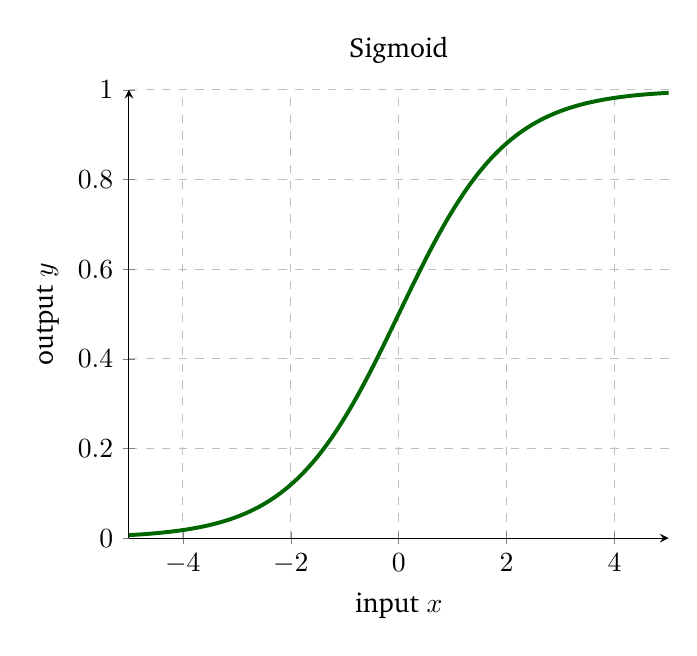
\begin{tikzpicture}
			\begin{axis}[
			title = {Sigmoid},
			axis lines = left,
			xlabel = {input $x$},
			ylabel = {output $y$},
			xmin = -5,
			xmax = 5,
			ymin = 0,
			ymax = 1,
			ymajorgrids=true,
			xmajorgrids=true,
			grid style=dashed
			]
			%Here the blue parabloa is defined
			\addplot [
			domain=-5:5, 
			samples=1000, 
			color=black!60!green,
			line width = 0.5mm
			]
			{1/(1+e^(-x))};
			
			\end{axis}
			\end{tikzpicture}
		}
		\caption{$\sigma(x)$}
		\label{img:activation_function_sigmoid}
	\end{subfigure}
	\begin{subfigure}[b]{0.3\textwidth}
		\centering
		\scalebox{0.5}{%
			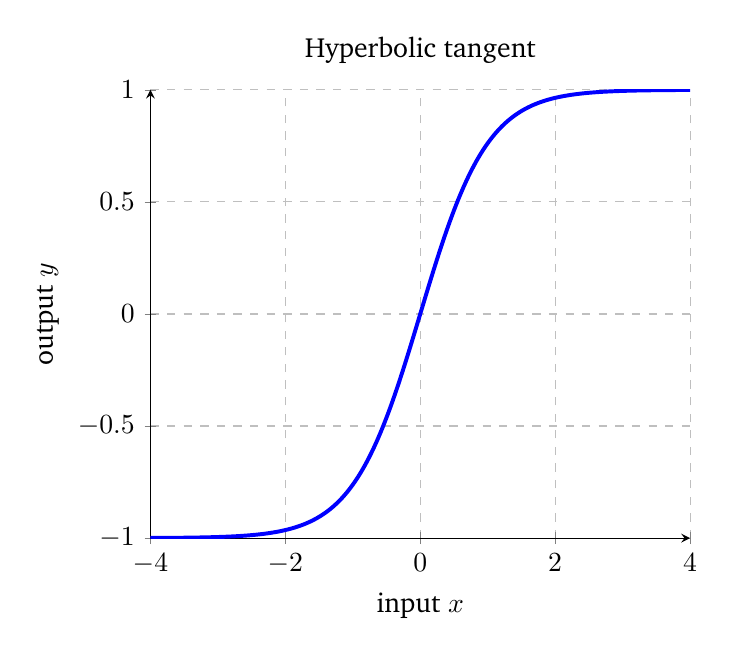
\begin{tikzpicture}
			\begin{axis}[
			title = {Hyperbolic tangent},
			axis lines = left,
			xlabel = {input $x$},
			ylabel = {output $y$},
			xmin = -4,
			xmax = 4,
			ymin = -1,
			ymax = 1,
			ymajorgrids=true,
			xmajorgrids=true,
			grid style=dashed
			]
			%Here the blue parabloa is defined
			\addplot [
			domain=-4:4, 
			samples=1000, 
			color=blue,
			line width = 0.5mm
			]
			{tanh(x)};
			
			\end{axis}
			\end{tikzpicture}
		}
		\caption{$\tanh(x)$}
		\label{img:activation_function_tanh}
	\end{subfigure}
	\begin{subfigure}[b]{0.3\textwidth}
		\centering
		\scalebox{0.5}{%
			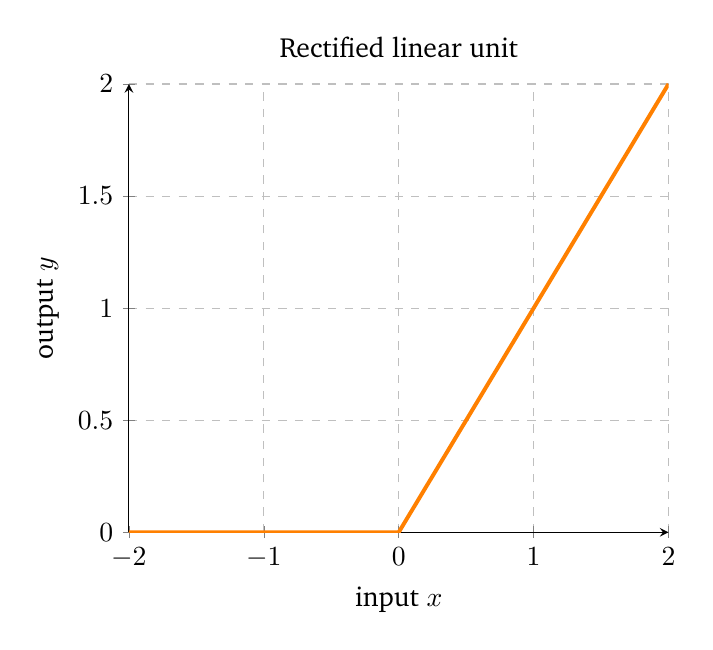
\begin{tikzpicture}
			\begin{axis}[
			title = {Rectified linear unit},
			axis lines = left,
			xlabel = {input $x$},
			ylabel = {output $y$},
			xmin = -2,
			xmax = 2,
			ymin = 0,
			ymax = 2,
			ymajorgrids=true,
			xmajorgrids=true,
			grid style=dashed
			]
			%Here the blue parabloa is defined
			\addplot [
			domain=-2:2, 
			samples=1000, 
			color=orange,
			line width=0.5mm
			]
			{(x > 0)*x};
			
			\end{axis}
			\end{tikzpicture}
		}
		\caption{$\text{ReLU}(x)$}
		\label{img:activation_function_relu}
	\end{subfigure}
	
	\caption[Comparison of activation functions]{(a) The sigmoid function maps the inputs to a range of 0 to 1 while having high gradients near to $y=0$ to bring the output more to either 0 or 1. (b) The hyperbolic tangent is similar to the sigmoid function but has a output range of -1 to 1. (c) A rectified linear unit (ReLU) is 0 for all input lower than 0. All other values are processed linearly so that they do not change.}
\end{figure}
\subsubsection{Hyperbolic tan}
Properties of the hyperbolic tan:
\begin{itemize}
	\item $\tanh(x) = \frac{e^{x} - e^{-x}}{e^{x} + e^{-x}}$
	\item $\tanh(-x) = -\tanh(x)$
	\item $\tanh'(x) = 1 - \tanh(x)^2$
	\item Output range: $[-1,1]$
\end{itemize}
\subsubsection{Softmax}
Properties:
\begin{itemize}
	\item $\text{softmax}(x_k) = \frac{\exp(x_k)}{\sum_{i=1}^{N}\exp(x_i)}$
	\item If $x_k \gg x_j$, the softmax for all $j\neq k$ is approx. 0, whereas for $k$ it is 1
	\item Maps vector from $\bm{y} \in \mathbb{R}^D$ to probability distribution $\bm{y}' \in [0,1]^D$ with $\sum_{i=1}^{D}y'_{i} = 1$ $\Rightarrow$ useful for multi-class classification
	\item Invariant to bias: $\frac{\exp(x_k + c)}{\sum_{i=1}^{N}\exp(x_i + c)} = \frac{\exp(x_k)}{\sum_{i=1}^{N}\exp(x_i)}= \text{softmax}(x_k)$
\end{itemize}
\subsection{Matrix operations}
\subsubsection{Properties of transposed and inverse matrices}
\textbf{Transpose}
\begin{itemize}
	\item $(AB)^T=B^T A^T$
	\item $\det\left(A^{T}\right) = \det\left(A\right)$
\end{itemize}
\textbf{Inverse}
\begin{itemize}
	\item $(AB)^{-1} = B^{-1} A^{-1}$
	\item $\det\left(A^{-1}\right) = \det\left(A\right)^{-1}$
\end{itemize}
\textbf{Combination}
\begin{itemize}
	\item $\left(A^{-1}\right)^T = \left(A^{T}\right)^{-1}$
\end{itemize}
\subsubsection{Derivations}
\subsubsection{Hand-in 1: 1.3d}
Derivation of multivariate Gaussian by matrix
\subsection{Lagrange Multiplier}
\begin{itemize}
	\item Finding stationary points of a function with subject to one or more constraints
	\item \textbf{Equality constraint}
	\begin{itemize}
		\item Maximize $f(\bm{x})$ with respect to constraint $g(\bm{x})=0$
		\item At a constrained maximum, we know that $\nabla f(\bm{x}) = -\lambda \nabla g(\bm{x})$
		\item The Lagrangian function is therefore $$ L(\bm{x}, \lambda) = f(\bm{x}) + \lambda g(\bm{x})$$
		\item We solve it by maximizing regarding to $\bm{x}$ and $\lambda$: $$\max_{\bm{x}} \max_{\lambda} L(\bm{x}, \lambda)$$
		\item Note that the sign of the constraint is irrelevant. A minus sign leads to the same result as $g(x)$ must be zero at this point
		\item We find solutions by setting the derivate of both primal and dual variables to 0:
		$$\frac{\partial }{\partial \bm{x}} L(\bm{x}, \lambda) = 0, \text{\hspace{3mm}} \frac{\partial }{\partial \lambda} L(\bm{x}, \lambda) = 0$$
	\end{itemize}
	\item \textbf{Inequality constraint}
	\begin{itemize}
		\item Maximize $f(\bm{x})$ with respect to constraint $g(\bm{x})\geq0$ (introduce Lagrangian multiplier $\mu$)
		\item Two kinds of solutions:
		\begin{itemize}
			\item If the optimum of $f(\bm{x})$ lies already in the region of $g(\bm{x})\geq0$, then we have an inactive constraint $\Rightarrow$ $\mu=0$
			\item Otherwise, the optimum is on the boundary so that $g(\bm{x})=$ and $\mu> 0$
		\end{itemize}
		\item Thus, our primal Lagrangian is defined as:
		$$L(\bm{x}, \mu) = f(\bm{x}) + \mu g(\bm{x})$$
		\item We now maximize regarding $\bm{x}$, but \textit{minimize} for the Lagrangian multiplier as we prefer $f(x)$ being inside the constraint area:
		$$\max_{\bm{x}} \min_{\mu} L(\bm{x}, \mu)$$
		\item Note that the sign is here important. When we minimize $f(x)$, we can keep the max-min conditions for the Lagrangian but then have to switch the sign in front of the constraint!
		\item Also, deriving by $\mu$ does not guarantee a valid solution anymore as we have the following KKT conditions for \textit{every} Lagrangian multiplier:
		$$\mu \geq 0 \hspace{5mm} g(\bm{x})\geq 0 \hspace{5mm} \mu g(\bm{x}) = 0$$
		\item We obtain the dual Lagrangian by optimizing with respect to only the primal variables $\bm{x}$, and replacing those in the primal Lagrangian:
		$$\tilde{L}(\mu) = \max_{\bm{x}} L(\bm{x},\mu)$$
		\item Next, minimize with respect to the dual parameters $\mu$ by considering the constraint $\mu=0$
	\end{itemize}
	\item \textbf{Combined constraints}
	\begin{itemize}
		\item If we have multiple constraints (can be pure (in-)equalities or mixed), we just add them all to our Lagrangian function
		\item Solve with respect to all constraints
	\end{itemize}
\end{itemize}
\end{document}